\documentclass[a4paper, 12pt]{scrartcl}

%===============================================================================
% Packages
%===============================================================================
\usepackage{fontspec}
\usepackage{geometry}
\usepackage[ngerman]{babel} % Use new german language definition
\usepackage{hyperref} % Hyperlinks in PDFs
\usepackage{amsmath, amsfonts, amssymb} % Math packages
\usepackage{graphicx} % For Graphics
\usepackage{xcolor} % For coloring texts
\usepackage{times} % Times New Roman Font
\usepackage{tikz} % The TikZ vector graphic library
\usepackage{fancyhdr} % Fancy headings
\usepackage{nameref} % References for names instead of numbers
\usepackage[absolute]{textpos} % Absolute positioning
\usepackage{titlesec} % Customizable ((Sub)Sub)Sections
\usepackage{titletoc} % Customizable ToC
\usepackage{tocloft} % Customizable ToC, LoF, …
\usepackage{pdfpages} % Embedding pdfs
\usepackage{wallpaper} % Background images
\usepackage{tikz-er2} % Entity relation diagrams
\usepackage{listings} % Code listings

%===============================================================================
% Tikz-Librarys
%===============================================================================
\usetikzlibrary{positioning}
\usetikzlibrary{shadows}

\tikzstyle{every node} = [font=\sffamily]
\tikzstyle{every entity} = [top color=kiba!10, bottom color=kiba!70, 
                            draw=kiba!80!black, drop shadow, font=\sffamily\bfseries]
\tikzstyle{every weak entity} = [drop shadow={shadow xshift=.7ex, 
                                 shadow yshift=-.7ex}]
\tikzstyle{every attribute} = [top color=white, bottom color=black!10, 
                               draw=black!50, node distance=1cm, drop shadow]
\tikzstyle{every relationship} = [top color=white, bottom color=red!20, 
                                  draw=red!50!black!100, drop shadow, font=\sffamily\itshape]
\tikzstyle{every isa} = [top color=white, bottom color=green!20, 
                         draw=green!50!black!100, drop shadow]
                         
%===============================================================================
% Listings
%===============================================================================
\lstset{
	emph={KBABranchDao, KBAAccountDao, KBACustomerDao, KBATransactionDao, KBAExchangeRateDao, KBACustomerDao, KBACreditRatingDao, KBAMessageDao, KBAAuth, KBADependencyInjector},
	emph={[2]NSString},
	language=[Objective]C, 
	morekeywords={new,@,},
	backgroundcolor=\color{black!3},
	columns=fullflexible,
	basicstyle=\ttfamily\footnotesize,
	keywordstyle=\bfseries\ttfamily\color{blue!50!red!80!black},
	stringstyle=\color{red!70!black}\ttfamily,
	identifierstyle=\ttfamily\itshape,
	commentstyle=\color{green!30!black}\ttfamily\itshape,
	emphstyle={\color{orange!70!black}\bfseries\texttt},
	emphstyle={[2]\color{green!60!blue!50!black}\bfseries\texttt},
	showstringspaces=false,
	flexiblecolumns=false,
	tabsize=4,
}

%===============================================================================
% Definitions
%===============================================================================
%\newcommand{\semantischerAusdruck}[1]{%
%	... was macht das ... #1

\newcommand{\Stichwort}[1]{%
	\textbf{#1}}
\setlength{\parskip}{6pt}
\renewcommand{\headrulewidth}{0pt}
\linespread{1.5}
\geometry{a4paper}
\geometry{left=25mm,right=25mm,bottom=30mm,top=30mm}
\geometry{footnotesep=10mm}
\geometry{headsep=10mm}
\geometry{head=10mm}
\geometry{bindingoffset=0mm}
\definecolor{kiba}{HTML}{41707C}
\newcommand{\pre}[1]{%
	\texttt{#1}}

%===============================================================================
% Collaborative
%===============================================================================
\definecolor{markus}{HTML}{FF3118}
\definecolor{alex}{HTML}{3152A5}
\definecolor{julius}{HTML}{639C18}
\definecolor{marco}{HTML}{844D18}
\definecolor{michael}{HTML}{A50063}
\definecolor{corny}{HTML}{0084A5}

\makeatletter
\def\name@markus{Markus Fasselt}
\def\name@alex{Alexander Droste}
\def\name@julius{Julius Wulk}
\def\name@marco{Marco F. Jendryczko}
\def\name@michael{Michael Schaarschmidt}
\def\name@corny{Konstantin S. M. Möllers}
\newcommand{\currentAuthor}{kiba}
\newcommand{\authoredSection}[2]{%
	\renewcommand{\currentAuthor}{#1}%
	\section[#2]{#2 {\normalfont\sffamily\small von \csname name@#1\endcsname}}}
\makeatother
\renewcommand{\lstlistingname}{Programmausdruck}

%===============================================================================
% Head / Foot
%===============================================================================
\pagestyle{fancy}
\fancyhf{}
\makeatletter
\fancyhead[L]{}
\fancyhead[R]{\sffamily\itshape Projektbericht „KiBa“-App}
\fancyfoot[C]{}
\fancyfoot[R]{\sffamily\thepage}
\makeatother

%===============================================================================
% Font
%===============================================================================
\setmainfont{Times}
\setsansfont[
	Extension = .ttf,
	Path = Fonts/,
	BoldFont = TheSansUHHBold,
	BoldItalicFont = TheSansUHHBolditalic,
	ItalicFont = TheSansUHHRegularItalic
]{TheSansUHHRegular}
\setmonofont[
	Extension = .otf,
	Path = Fonts/,
	BoldFont = lmmonolt10-bold,
	BoldItalicFont = lmmonolt10-boldoblique,
	ItalicFont = lmmonolt10-oblique
]{lmmono12-regular}

%===============================================================================
% Sections
%===============================================================================
\titleformat{\section}[hang]{\Large\sffamily\bfseries\color{\currentAuthor}}{\thesection\quad}{0pt}{}
\titleformat{\subsection}[hang]{\large\sffamily\itshape}{\thesubsection\quad}{0pt}{}
\titleformat{\subsubsection}[hang]{\large\sffamily}{\thesubsection\quad}{0pt}{}

%===============================================================================
% Table of Contents
%===============================================================================
\renewcommand{\cftfigpresnum}{Abb. }
\renewcommand{\cfttabpresnum}{Tab. }
\renewcommand{\cftfigaftersnum}{:}
\renewcommand{\cfttabaftersnum}{:}
\setlength{\cftfignumwidth}{2cm}
\setlength{\cfttabnumwidth}{2cm}
\setlength{\cftfigindent}{0cm}
\setlength{\cfttabindent}{0cm}

\def\tocindent{15mm}
\titlecontents{section}[\tocindent]{\vspace{10pt}\sffamily\bfseries}{\noindent\contentslabel{\tocindent}}%
	{\hspace*{0cm}}{\hfill\contentspage}
\titlecontents{subsection}[\tocindent]{}{\noindent\contentslabel{\tocindent}}%
	{\hspace*{0cm}}{\hfill\contentspage}
    
%===============================================================================
% Meta Description
%===============================================================================    
\author{%
	Alexander Droste\vphantom{yMö}\\[-2pt]
    Markus Fasselt\vphantom{yöM}\\[-2pt]
    Marco F. Jendryczko\vphantom{yMö}\\[-2pt]
    Konstantin S. M. Möllers \vphantom{yMö}\\[-2pt]
    Michael Schaarschmidt\vphantom{yöM}\\[-2pt]
    Julius Wulk\vphantom{yMö}}
\title{Die „KiBa“-App}
\date{Wintersemester 2013/14}

    
%===============================================================================
% Document
%===============================================================================
\begin{document}
	
\makeatletter
\thispagestyle{empty}

\begin{center}
	\textcolor{kiba}{\bf\sffamily\fontsize{48pt}{48pt}\selectfont \@title} \\[.5cm]
	
\includegraphics[height=3cm]{logo-kiba} \\[.5cm]
	\textcolor{kiba}{\LARGE\sffamily Projektbericht} \\[.5cm]
    {\large\sffamily Angefertigt von} \\[4pt]
    {\Large \@author \\[1.5cm]}
    {\large\sffamily Veranstalter} \\[12pt]
    {\Large Dr. Guido Gryczan} \\[6pt] {\LARGE Dr. Martin Christof Kindsmüller\vphantom{y}} \\[6pt] {\LARGE Christian Zoller} \\[1.5cm]
    {\Large\sffamily \@date}
\end{center}

\vspace{2.5cm}

% UHH-Logo
\begin{textblock*}{85mm}(20mm, 257mm)
	
\includegraphics[width=2cm]{logo-uhh}\;{\sffamily Universität Hamburg}
\end{textblock*}

% FBI-Logo
\begin{textblock*}{85mm}(105mm, 257mm)
	\hfill{\sffamily Fachbereich Informatik}\;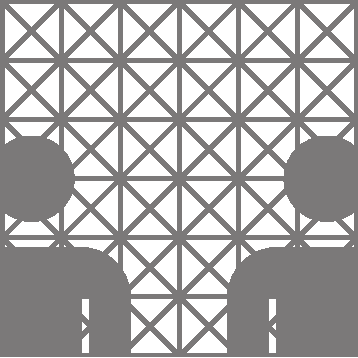
\includegraphics[width=2cm]{logo-fbi}
\end{textblock*}

\makeatother
\newpage
    
\tableofcontents
\newpage

%===============================================================================
% Parts
%===============================================================================
\section{Aufgabenstellung und Vision}
	Die unser Gruppe übertragene Aufgabe bestand darin, eine iOS-App zu entwickeln, die die Bindung zwischen einer fiktiven Filialbank und ihren Kunden erhöht. In den ersten Ü\-ber\-le\-gung\-en wurde schnell deutlich, dass nahezu jede Dienstleistung einer Filiale auf die ein oder andere Weise von Direktbanken abgebildet werden kann. Das Alleinstellungsmerkmal besteht im direkten menschlichen Kontakt vor Ort und in der persönliche Bindung zu einem möglicherweise vertrauten Berater. 
    
Insofern haben wir uns nach einem Prozess von abwechselnden Gruppendiskussion und externen Feedback dazu entschlossen, diejenigen Features zu betonen, die Berater und Kunden möglichst in der Filiale zusammenbringen, aber auch unabhängig davon genutzt werden können. Auch Direktbanken versuchen inzwischen, anonyme Hotlines zu vermeiden und Kunden einzelnen Beratern zuzuordnen. In Kombination mit niedrigeren Gebühren, kostenlosen Kreditkarten und einfacher Kontoführung ist dies ein schwer zu schlagendes Angebot. Eine App, die Neukunden für eine Filalbank gewinnen soll, muss also einerseits eine ähnlich einfache Kontoverwaltung bieten, außerdem aber noch einen Mehrwert schaffen, der die höheren Gebühren einer Filialbank rechtfertigt.

Ein weiterer, für die Akzeptanz einer App wichtiger Aspekt ist die (vielleicht auch nur vom Kunden gefühlte) Sicherheit. Eine von uns durchgeführte Umfrage unter Studenten technischer Fächer, primär Informatik, ergab, dass die meisten Teilnehmer unabhängig von der Funktionalität schon aus Sicherheitsgründen keine Bankgeschäfte mit einer App erledigen wollten. Die besondere Sensibilität der genannten Zielgruppe für Sicherheitsaspekte darf nicht außer Acht gelassen werden; dennoch ergab sich für uns die Frage, ob hier durch Interaktion in der Filiale nicht zugleich Kundenbindung und Vertrauen in die Sicherheit der Anwendung erhöht werden könnten. 

Insgesamt entstand also die Vorstellung einer Anwendung, die klassische Bankgeschäfte wie Überweisungen beherrscht, gleichzeitig aber versucht, Lokalität und Interaktion mit dem eigenen Berater herzustellen. 
\authoredSection{michael}{Kontext und App-Idee}
\subsection{Name}
    Der Name der App, "`\textbf{K}i\textbf{B}a"', steht in Anlehnung an eine bekannte Direktbank für eine kundeninteressierte Bank, die mit der Anwendung mehr über ihre Kunden erfahren möchte und mit ihnen in Austausch treten will, um spezifischere Angebote und Beratungen anbieten zu können.
    
\subsection{Gerät}
    Bei der Erstellung eines konkreten Konzepts der Funktionalität haben wir zunächst die Anwendungsfälle besprochen, um die Gerätfrage zu klären. Zweifelsohne gibt es Features, die in einem mobilen Anwendungsfall wahrscheinlicher sind, etwa das Auffinden einer Filiale oder eines Geldautomaten. Eine solche Funktionalität wäre aber nicht filialbankspezifisch. Überhaupt erschien es uns, als wäre der typische Anwendungsfall eher stationär, auf dem Sofa, im Büro, jedenfalls aber in Ruhe. Ein überzeugendes Argument für eine iPad-App ist auch, dass Kunde und Berater in der Filiale zusammen mit der App interagieren und Dinge visualisieren können. Die Vorstellung, ein Kreditangebot auf dem Bildschirm eines iPhones durchzusprechen, ist hingegen eher absurd. 
    
    
    Somit überwogen in der Gruppe ganz eindeutig die Argumente für eine iPad-Anwendung. Zudem war es Aufgabe, eine Vision für die Banking-App der Zukunft zu entwickeln. Der Trend geht unserer Meinung nach zum ubiquitären W-Lan; so gibt es beispielsweise Bestrebungen, öffentliche Netzwerke in der Innenstadt einzurichten. Insofern darf davon ausgegangen werden, dass die mobile Konnektivität zukünftig auch beim iPad zukünftig unproblematisch ist und somit webbasierte Funktionalität auch unterwegs gegeben ist.
    

\subsection{Funktionen}
    Die Kernfunktionen der App sollen sich auf genau die Bereiche konzentrieren, die einer Direktbank nicht zur Verfügung stehen und somit nicht trivial nachgebaut werden können. Dabei haben wir im Zuge der Plenumsdiskussionen und anschließenden internen Debatten insbesondere den zeitlichen Aspekt als zentrale Komponente identifziert. Viele Bescheinigungen und Unterlagen im täglichen Leben werden auch heute noch konkret ausgedruckt benötigt. Der typische Ablauf einer Direktbank sieht so aus, eine Anfrage (etwa nach Wertpapierzweitschriften) per Kontaktformular abzuschicken und dann einige Tage auf die entsprechenden Ausdrucke zu warten. Unsere Idee besteht in einer Self-Service Station innerhalb der Bank, die das Konzept bestehender Automaten erweitert. Ein Kunde kann sein Ipad auf eine Ablage legen und sich mit der Station verbinden. Die Station beinhaltet einen Multifunktionsdrucker und per App können verschiedenste Bescheinigungen ausgedruckt werden. 
    
    Ein wesentliches Produkt von Filialbanken ist das klassische Sparbuch. Umbuchungen können üblicherweise nur in einer Filiale vorgenommen werden, überwiesen werden kann nur auf das Sparkonto. Die Greifbarkeit des Sparbuches vermittelt konservativen, besorgten Sparern ein Gefühl von Sicherheit. Gleichzeitig kann es aber durch diese funktionale Einschränkung auch zu unerwünschten Situationen kommen: ist etwa durch eine Fehlkalkulation an einem Samstagabend kein Geld mehr auf dem Girokonto, muss bis zur Öffnung einer Filiale am Montag gewartet werden, um Guthaben umbuchen zu können. Um dem Vorzubeugen, soll über die Self-Service Station auch Geld umgebucht werden können. Da die Station im Vorraum der Filiale steht, ist sie ganztägig zugänglich. Auf diese Weise bleibt einerseits das Sparbuch als vertrauenswürdige Marke erhalten, die in der Wahrnehmung misstrauischer Benutzer von den Verwerfungen der Online-Kriminalität unberührt bleibt, andererseits ist die Verfügbarkeit erheblich verbessert.
    
    Ebenfalls auf die Bereitstellung von Service-Dienstleistungen zielt der interaktive Filialfinder ab. Aus der Karte heraus sollen Anfragen an eine bestimmte Filiale in der Umgebung er möglicht werden, indem etwa ein Beratungstermin reserviert wird und dann ohne Anstehen erfolgen kann. Eine Funktionalität dieser Art ist 
      
    Als Startbildschirm für die App ist ein Dashboard vorgesehen, das einen graphischen Überblick über Vermögensverlauf und Transaktionen bereitstellt. Hilfreich war hier die Überlegung, dass die meisten Benutzer ihren Kontostand grob kennen und weniger an einer Zahl als vielmehr an den Entwicklungen interessiert sind. Ist der Benutzer nicht eingeloggt, erscheint an dieser Stelle ein Mockup mit der Aufforderung, sich einzuloggen.
    
    Das Kerngeschäft von Filialbanken besteht in der Finanzierung, etwa für Eigenheime. Im Zentrum unserer Überlegungen stand dann auch die Frage, wie eine App dabei helfen kann, diese Dienstleistung für den Endkunden zu verbessern. Im Ergebnis möhten wir einen individualisierten Kreditrechner anbieten, der den App-Benutzer in die Lage versetzt, mittels individuell berechneter Profildaten für sich selbst Finanzierungsrechnungen durchzuführen. Die Idee dahinter ist, dass ein Kunde zunächst für sich selbst einige Finanzierungsvarianten durchspielen kann. Hat er sich eine Variante überlegt, kann ein Termin mit dem persönlichen Berater vereinbart werden und dabei optional gleich der Finanzierungsvorschlag exportiert werden. Im Filialgespräch kann der Berater dann noch individuelle Ratschläge bezüglich Laufzeit und Umfang einer Finanzierung geben.
    
	Eng zusammenhängend mit dem Finanzierungsprofil steht die Aktivierung ("`Authentifikation"') der App in einer Filiale. Ohne eine solche Aktivierung steht dem Benutzer nur passive Funktionalität zur Verfügung, also etwa der Filialfinder und die Umsatzanzeige. Um die App voll nutzen zu können, muss der Benutzer in eine KiBa-Filiale und von einem Berater einen Sicherheitscode eingeben lassen. Ähnlich einer Kreditkarte soll dann bei Gerätverlust auch die App selbst jederzeit gesperrt werden können. Insbesondere dient die Aktivierung aber auch dazu, den Kunden in einem Beratungsgespräch besser kennenzulernen und in einer bankseitigen Datenbank einen persönlichen Ansprechpartner festzuhalten. Aus der App kann dann direkt ein Termin mit dem eingetragenen Berater vereinbart werden. Auch ein Nachrichten-System ist denkbar, um einzelne Fragen direkt zu klären.
\authoredSection{julius}{Mockups}

\authoredSection{alex}{Vorgehen}
\subsection{Orientierungsphase}
	Zu Beginn des Vorgehens standen Ideenfindung, Konzeption, Lernprozesse und das Finden eines gemeinsamen Arbeitsrhythmusses im Vordergrund. Eine erste grobe Orientierung, welche Aufgabenteile die einzelnen Beteiligten der Gruppe im Verlauf annehmen würden, ergab sich nach der „Kick-Off“-Veranstaltung bei T-Systems. Die Kompetenzen des Teams wurden anschließend auf die Positionen des Entwicklers, Konzepters, Projektleiters und Beraters aufgeteilt. 
	
	Zum Zeitpunkt der Ideenfindung wurde das Vorgehen noch weniger zentral organisiert, als es später durch den Projektleiter realisiert werden sollte. Es galt zunächst herauszufinden, mit welchen konkreten Aufgaben man sich im weiteren Verlauf konfrontieren konnte. Um eine grundlegende Kommunikation zwischen den Teammitgliedern zu etablieren, wurde eine Facebook-Gruppe gegründet, die dazu diente Ideen festzuhalten, zu besprechen und Termine oder Aufgaben für kommende Treffen zu vereinbaren. Um die Ideen darüber hinaus geordnet aufzuschreiben und für alle Beteiligten abrufbar zu machen, wurde zusammen mit dem Coderepository ein Wiki bei Github angelegt, siehe Abbildung \ref{fig:WikiHome}. Das Wiki fand im Speziellen in dieser frühen Phase Verwendung.
	
\begin{figure}[h]
	\centering
	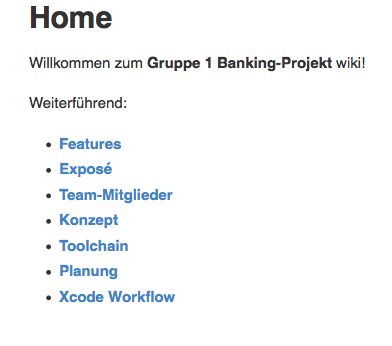
\includegraphics[width=6cm]{Pictures/wiki_home}
	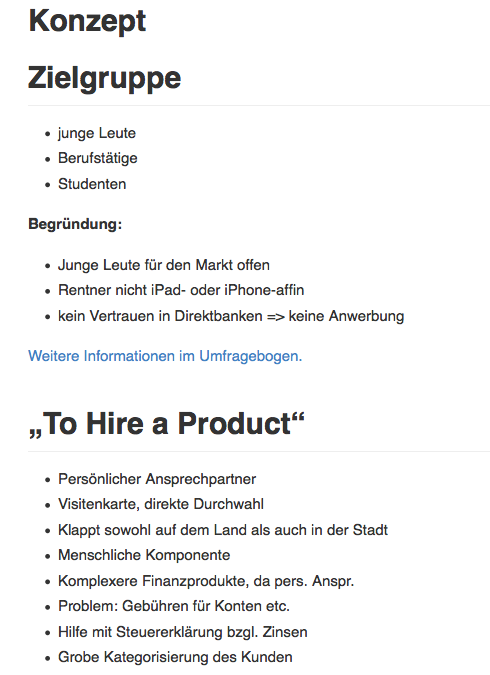
\includegraphics[width=6cm]{Pictures/wiki-konzept}
	\caption{Wiki bei Github\label{fig:WikiHome}}
\end{figure}

	Neben der Formfindung von Konzepten diente das Wiki ebenfalls zum Festhalten von Code-Style Konventionen (NYTimes Objective-C-Style Guide) oder Workflows, wie etwa dem toolunterstützten Erstellen von Doxygen-kompatiblen Methodenkommentaren mit dem Xcodeplugin VVDocumenter\footnote{\url{https://github.com/onevcat/VVDocumenter-Xcode}}. Auf Basis des Letzterem ließe sich bei Bedarf aus den Kommentaren eine Dokumentation im html-Format generieren. 

	Einen der ersten Schritte im Arbeitsprozess nach Erstellung des Exposés konnten wir mit Hilfe einer Umfrage bezüglich der Kundenbedürfnisse, -erwartungen und -bedenken respektive des Genres der Applikation, sowie unserer spezifischen Vorstellung, sprich der möglichen Features des Endprodukts, erreichen. Im Rahmen der ersten internen Treffens des Teams und der Plenumsveranstaltungen konnten sich die Vorstellungen langsam konkretisieren. Deutlich wurde dabei, wie diese zu priorisieren sind und welche Einschränken (wie bspw. Sicherheitsaspekte, Wertigkeit des Features) an eine mögliche Umsetzung geknüpft sind. In diesem Prozess wurde das Konzept stetig auf die Rückmeldungen der Plena angepasst. Begleitet wurde das Vorgehen durch das Erstellen von Mockups, die bereits in diesem Stadium helfen konnten, Inhalte nicht zuletzt visuell zu vermitteln und zu besprechen. Die Verwendung von Mockups fand aber auch im weiteren stets Anwendung, um Skizzen für eine mögliche Visualierung zu erstellen, bevor diese final umgesetzt wurden.

	Besonderes Augenmerk lag in der frühen Phase bezogen auf das Konzept im Herausarbeiten eines Alleinstellungsmerkmals, durch das sich mit Hilfe der Applikation die Fililalbank von der Direktbank positiv abheben kann. Dieser Punkt markierte gewissermaßen bei unserem Team die Hürde, um mit der eigentlichen Umsetzung zu beginnen. Die Featureideen sortierten wir fortlaufend neu nach geschätzter Priorität. Im Wiki unterschieden wir dabei grundsätzlich zwischen „Major“ und „Minor“.  
	
	Mit den Major-Features sollten die Kernfunktionalitäten der Applikation beschrieben werden. Hierzu zählten unter anderem der Filialfinder, der individuell angepasste Kreditrechner, sowie später primär fokussiert der Self-Service. Features, welche die App in der Gesamtheit aufwerten sollten aber nicht zur Kernfunktionalität gehören, bildeten die Minor-Kategorie. Ein Beispiel hierfür ist die Überweisungsfunktion für Girokonten. Sie wird in diesem Kontext erwartet, stellt aber keine Möglichkeit zur Abgrenzung gegenüber ähnlichen Anwendungen dar. Sie trägt außerdem nicht direkt dazu bei, die übergeordnete Fragestellung den Kunden wieder mehr an die Filialbank zu binden, zu erfüllen. Im Rahmen der Priorisierung verdeutlichte sich des weiteren, welche Features später nicht umgesetzt würden. Ein Feature das aufgrund niedrig eingestufter Priorität nicht den Weg bis in das Endprodukts geschafft hat, ist bspw. der SEPA-Umrechner, der das zuvor bestehende Format in die neue Kodierung umrechnen sollte. 
	
	Ebenfalls gab ausgedehnte Überlegungen, ob die Software für iPad, iPhone oder sogar dual für beide Geräte entwickelt werden sollte. Wie bei den Features war es auch hier hilfreich, wenn auch nicht einfach, demokratisch über eine Entscheidung abzustimmen. Dies zog auch nach sich, dass das Kollektiv den Einzelnen teils entgegen seiner eigenen Überzeugung zu einer gemeinsamen Lösung drängte. 
	
	Da die Kernfrage der Kundenbindung an die Filialbank schwer zu beantworten war, kam die Fragestellung des Zielgeräts und der damit verbundenen Auswahl an Features nach einer zuvor vermeintlich finalen Entscheidung mehrmals auf. Schlussendlich fiel die Entscheidung auf das iPad, weil wir die Kernfeatures durch dieses besser abdeckt sahen und sich nach der Umfrage der Eindruck einstellte, dass Nutzer sicherheitskritische Anwendungen bevorzugt in Ruhe Zuhause statt unterwegs verwenden wollen. Der Entschluss, sich bei der Entwicklung auf ein Gerät zu fokussieren, wurde teamintern unter den Gesichtspunkten mangelnden Gewinns einer dualen Entwicklung und dem damit verbundenen zusätzlichen Aufwand entschieden.

\subsection{Umsetzungsphase}
	Nachdem das grundlegende Konzept ausgearbeitet war, konnten wir mit der konkreten Umsetzung beginnen. Infolgedessen musste sich das Team auf einen Satz von Tools einigen, mit denen die Entwicklungsaufgaben verwaltet, zugeteilt und festgehalten wurden. Initial fiel die Entscheidung auf eine Kombination von Google-Docs und Github-Issues/Milestones. In Github lassen sich sog. Issues definieren. Diese Issues stellen Aufgaben dar, die Mitgliedern des Teams zugewiesen werden. Einzelne Issues werden wiederum Zwischenzielen zugewiesen, den Milestones. Sind alle Issues bezüglich eines Milestones abgearbeitet, ist dieses erfüllt. Die Verwaltung und Verteilung der Aufgaben wurde von diesem Zeitpunkt an durch den Projektleiter zentral durchgeführt. Alle neu entstehenden Aufgaben wurden also immer in Absprache mit diesem in das Issuesystem eingefügt. Dies war für die Übersicht der kommenden Aufgaben, verbunden mit der Gewissheit, dass alle Mitglieder über den Fortschritt im Ganzen wie im Einzelnen den gleichen Informationsstand haben, eine echte Hilfe. Die in Github eingetragenen Issues wurden neben der Zuweisung an Personen mit Labels versehen, die zum einen die Priorität zum anderen, das Überthema der Aufgabe beschreiben. Hochprior wurde u. a. das Erstellen einer Basisarchitektur auf der im weiteren softwaretechnisch aufgebaut werden sollte, sowie das Beschreiben der vorkommenden Entitäten und der damit verbundenen Relationen eingestuft. 

	Während wir GitHub zum Zuteilen und Festhalten der Aufgaben einsetzten, konnte mit Google-Docs der zeitliche Aufwand dafür festgehalten werden. Pro Aufgabe wurde eine Zeile mit entsprechendem Titel angelegt. Falls vorhanden, ist in der Tabelle das korrespondierende GitHub-Issue mit Verlinkung eingetragen. Die den Aufgaben zugewiesenen Teammitglieder sind mit Initialen vermerkt. Aus der tatsächlich aufgewendeten Zeit multipliziert mit der Anzahl der zugeteilten Personen resultiert der kumulierte Aufwand. Die Vorstellung der zu erledigenden Arbeiten war zu diesem Zeitpunkt allerdings meist unvollständig konkretisiert. Davon abgesehen gab es keine Vorerfahrungen bezüglich des iOS-Frameworks. Entsprechend mussten wir davon ausgehen, dass Aufwandsschätzungen zu Beginn nur bedingt hilfreich sein konnten. Trotzdem war dies als Vorlauf evtl. wichtig, um im  weiteren Verlauf ein gutes gemeinsames Verständnis für die Dokumentation und Verwaltung des Arbeitsaufwands zu entwickeln und zu präzisieren. 

\begin{figure}[h]
	\centering
	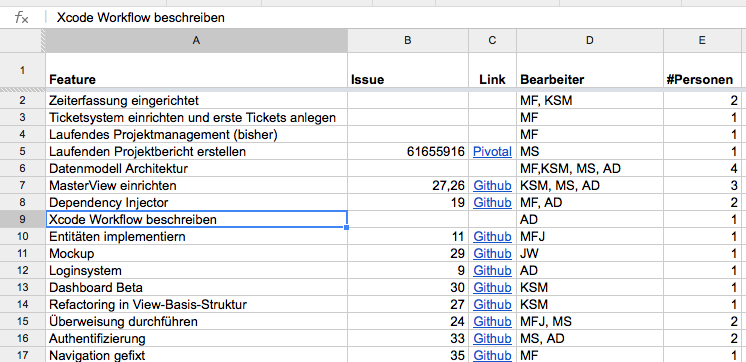
\includegraphics[scale=.25]{Pictures/gdocs1} \\
	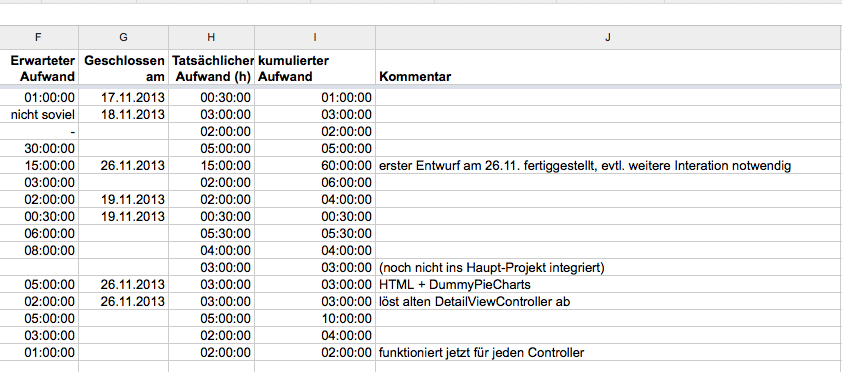
\includegraphics[scale=.25]{Pictures/gdocs2}
	\caption{Google Doc\label{fig:GDoc}}
\end{figure}

	Während der Anfangsphase etablierte sich im Team ein Arbeitsrhythmus mit zwei Terminen pro Woche, in denen jeweilig das Arbeitspensum eines Werktages oder darüber hinaus absolviert wurde.  Die zeitlichen Gegebenheiten mussten auf unsere Gruppe von Studenten mit je unterschiedlichen Stundenplänen abgestimmt werden. In voller Gruppenstärke war es, abgesehen von Ausnahmen, folglich kaum möglich, außerhalb der festen Projekttermine zusammenzukommen. Um in unseren Arbeitsabläufen dennoch Kontinuität herzustellen, haben wir die vereinbarten Termine entsprechend organisiert, dass mindestens die Hälfte der Gruppe anwesend sein konnte. Folglich wurden die Termine alternierend in unterschiedlichen Besetzungen durchgeführt. 

	Die frühen Teamtreffen waren neben den eigentlichen Aufgabenstellungen stark davon geprägt, sich mit Objective-C, dem iOS-Framework sowie der Entwicklungsumgebung vertraut zu machen. Vielleicht wurde auch infolge dessen zunächst primär eine technische Umsetzung unter Vernachlässigung visueller Aspekte versiert. Nach der Rückmeldung in einem der frühen Plenumstermine, dass visuelle Gestaltung der technischen zeitlich nicht nachsteht und parallel dazu entwickelt werden sollte, wurde die Arbeitsweise dahingehend umgestellt. Technische und visuelle Gestaltung wurden von diesem Zeitpunkt an gleichzeitig entwickelt. 

\subsection{Vorgehensweise nach Scrum}
	Im Anschluss an die Scrum-Zertifizierung wurden Arbeitsabläufe und Positionierung der Mitglieder im Team erneut reflektiert, um einen Scrum-Prozess mit den entsprechenden Rollen zu realisieren. Korrespondierend zu den zuvor zugewiesenen Positionen des Entwicklers, Projektleiters, Beraters und Konzepters wurde nach Äquivalenten in der Scrum-Terminologie gesucht. Entwickler und Konzepter wurden der Gruppe des Development Teams zugeteilt. Während beim Berater eine Analogie zum Scrum Master gebildet wurde, lag es nahe, den Projektleiter dem Product Owner zuzuordnen. 

	Bereits vor der Zertifizierung hatte sich durch den Scrum Master die Praxis eines Daily Scrums eingestellt. Das Daily Scrum Meeting wurde immer zu Beginn jedes Treffens umgesetzt. Dies brachte den positiven Effekt mit sich, dass trotz alternierender Besetzungen sich alle Mitglieder zu Arbeitsbeginn über den aktuellsten Stand ausgetauscht hatten. Der Product Owner zuvor Projektleiter verwaltete weiterhin wie zuvor beschrieben zentral das Aufgabenmanagement. 
Problematisch erwies sich die zuvor getroffene Toolauswahl zur Organisation der Aufgaben unter den Gesichtspunkten von Scrum. Primär fehlte es den Tools an Möglichkeiten der Idee des iterativen Sprints gerecht zu werden. Infolgedessen stellte das Team die gesamte Toolchain zur Verteilung der Aufgaben und deren Aufwandsmessung um. Die Wahl fiel auf das Tracking-Tool PivotalTracker, in welchem die Terminologie Scrums mit Sprint-Backlog, Sprint-Velocity, „Done“- Status, usw. vertreten war. Die zuvor erstellten Issues und Aufwandseinschätzungen der noch offenen Aufgaben wurden komplett in die neue Umgebung übertragen.

\begin{figure}[h]
	\centering
	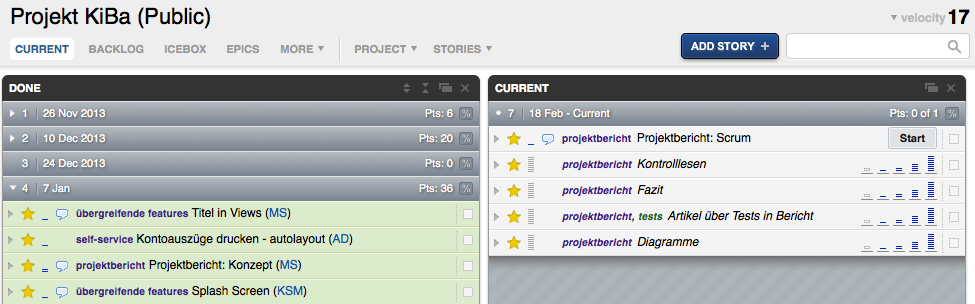
\includegraphics[scale=.25]{Pictures/pivottracker-overview}
	\caption{Stories bei PivotalTracker\label{fig:Pivottracker}}
\end{figure}

	Als Iterationsdauer legten wir einen Zeitrahmen von zwei Wochen fest. Diese Dauer erschien uns als sinnvoll; einerseits lang genug um, kleine oder mittelgroße Aufgaben innerhalb einer Iteration zu bewerkstelligen, anderseits nicht zu lang, um dynamisch auf geänderte Anforderungen reagieren zu können, ohne den Sprint-Backlog innerhalb eines Sprints modifizieren zu müssen. 
	
	Der Prozess des dynamischen Reagierens auf Kritik und sich damit ändernden Anforderungen vollzog sich über die gesamte Zeitspanne des Projekts. Das stetige Überdenken und Anpassen voriger Überlegungen und Ausarbeitungen stellte sich als eine der größten, wenn nicht als die größte Herausforderung des Projekts dar. Eine ständige Korrektur führt auch zum Verwerfen voriger Arbeit, woraus die Anforderung entsteht, sich stetig für neue Richtungswechsel zu motivieren.  

	Nach der Anfangsphase wurden die Aufwandsschätzungen präziser. Weiterhin war es zwar schwierig, genaue Schätzungen für einzelne Aufgaben vorzunehmen, insgesamt konnten wir aber trotz alledem auf Basis der sich ergebenden Sprint-Velocity ab dem letzten Drittel des Semesters eine sinnvolle Einschätzung über den verbleibenden Arbeitsaufwand und die dafür benötigte Zeit abgeben. Wie sich herausstellte, konnten wir diese Einschätzung auch einhalten. 

	Bezüglich der strengen Richtlinien von Scrum – entweder es wird auf voller Linie praktiziert oder aber das Vorgehensmodell ist nicht eingehalten und somit auch anders zu benennen – ist noch erwähnenswert, dass diese eigentlich vorsehen, dass das Development Team zu Beginn seiner Arbeit bereits alle notwendigen technischen Kompetenzen zur Umsetzung eines Projekts besitzt. Wir waren allerdings damit konfrontiert, selbstständig fortlaufend Wissen zu erarbeiten, das zur Bewältigung der Aufgaben notwendig war.

	 Neben den erwähnten Vorteilen des Tracking-Tools, respektive Struktur und Terminologie, ermöglichte uns die neue Umgebung das Verhältnis von bestehenden und noch zu erledigenden Aufgaben in Balkendiagrammen und Burndown-Charts zu visualisieren. Der Burndown-Chart bzw. Progress-Report über die gesamte zweite Hälfte der Projektdauer ergibt sich wie folgt:
	 
\begin{figure}[h]
	\centering
	\hspace{1.6cm}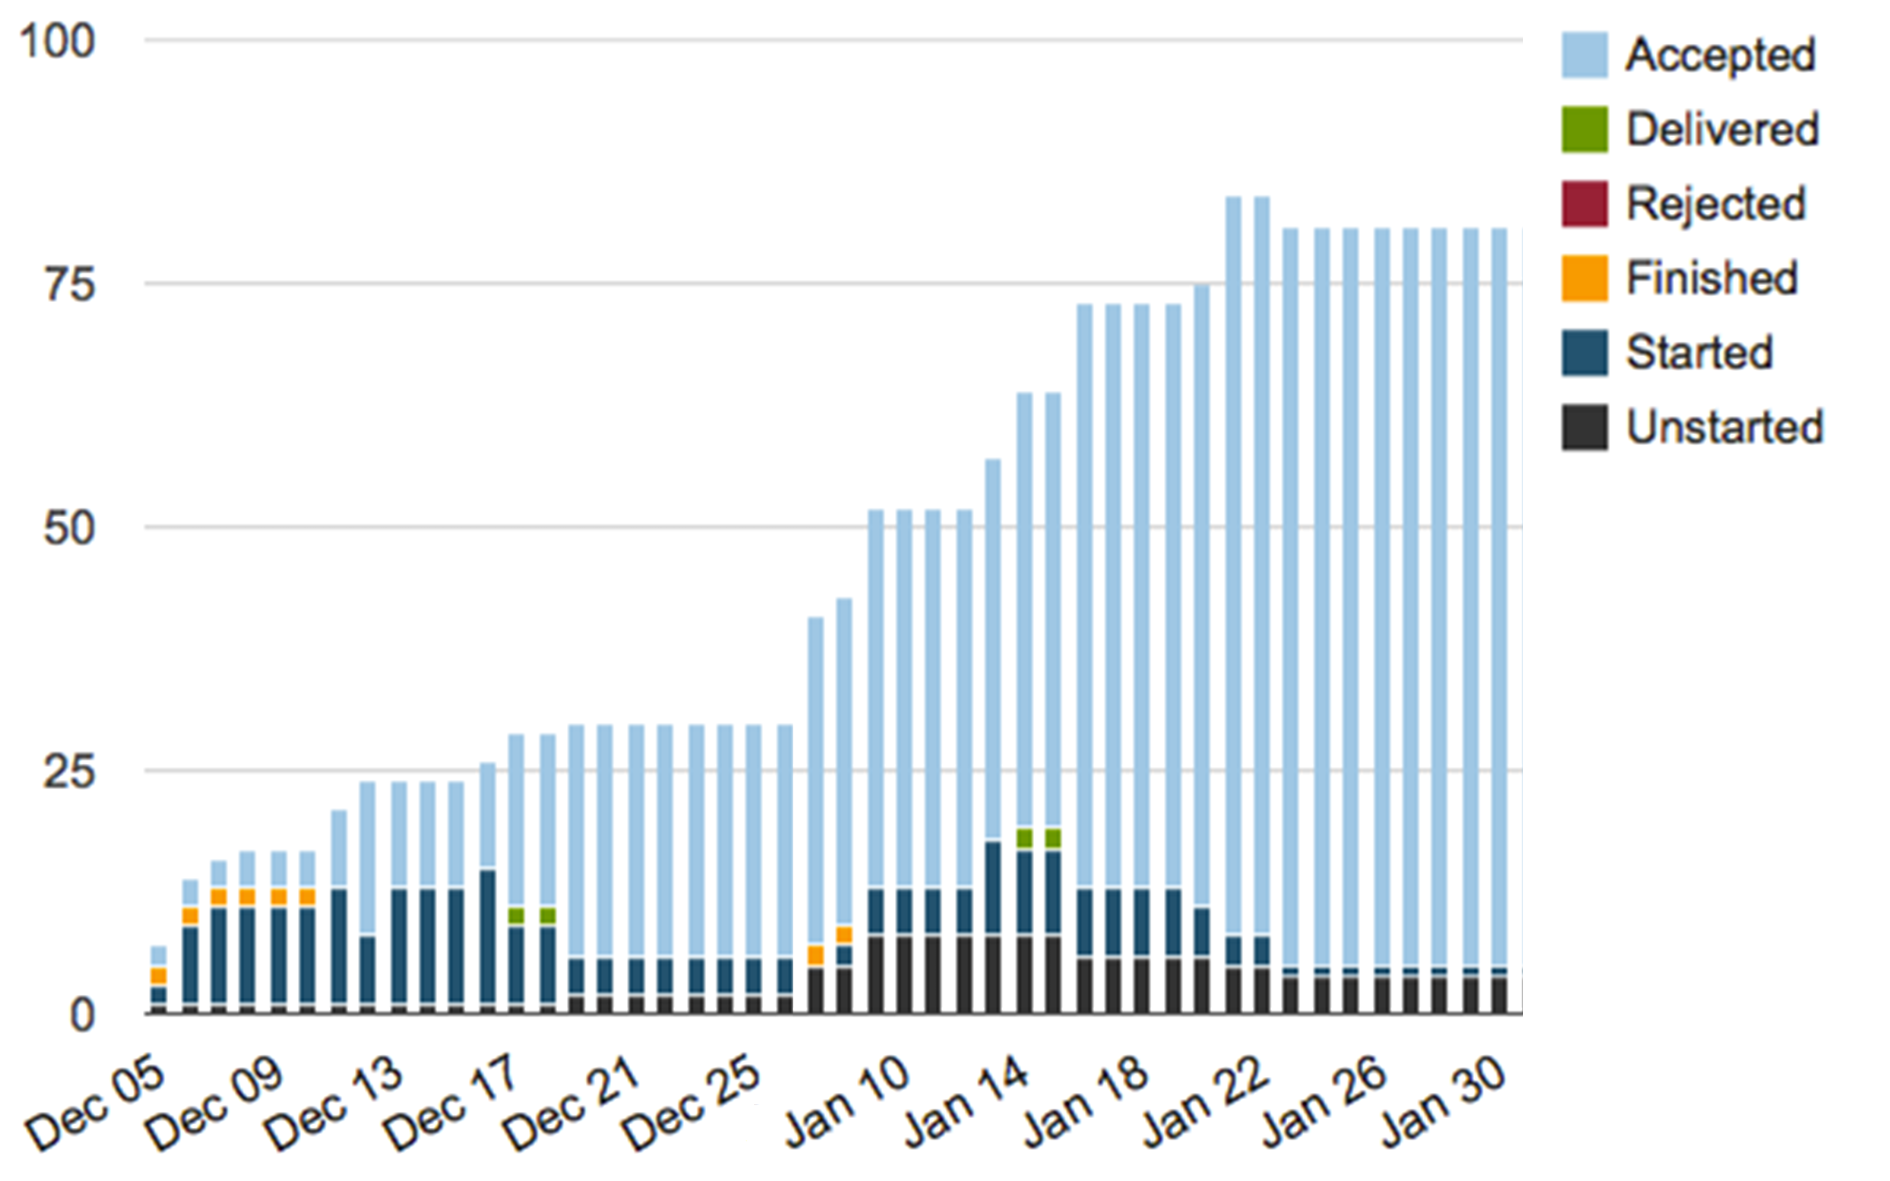
\includegraphics[width=.6\textwidth]{Pictures/burndown-compiled}
	\caption{Von PivotalTracker generiertes Burndown-Chart \label{fig:BurndownCompiled}}
\end{figure}

	Aus der Tendenz ist ersichtlich, dass die Sprint-Velocity unter Vernachlässigung der Ferienzeit stetig  bis zur Deadline zunahm.
\section{Design}
\authoredSection{marco}{Ergebnis}
\vspace{-24pt}
\subsection{Features}
\subsubsection{Dashboard}
\begin{figure}[h!]
	\centering
  	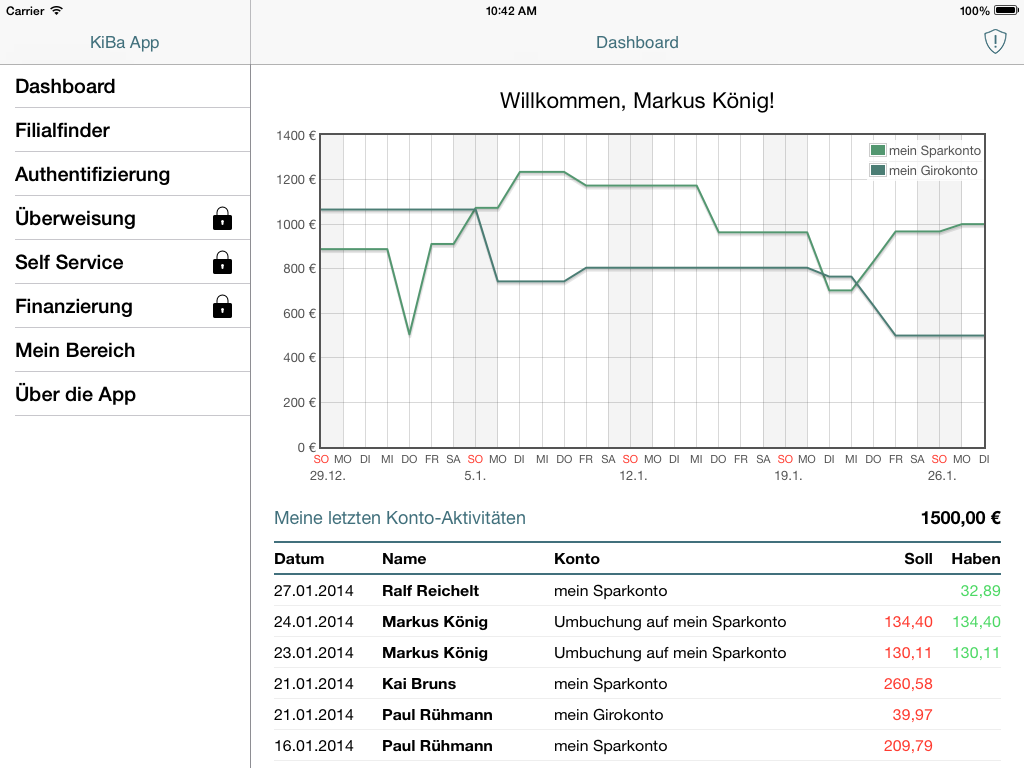
\includegraphics[height=0.25\textheight]{Pictures/Dashboard}
	\vspace{-12pt}	
	\caption{Screenshot des Dashboards}
	\label{fig1}
\end{figure}

Das Dashboard ~\ref{fig1} ist die zentrale Anlaufstelle der Applikation; dort haben wir einen Überblick über den Verlauf der Kontostände aller unserer Konten. In der Tabelle darunter haben wir die Möglichkeit, alle Kontobewegungen nachzuverfolgen.

\subsubsection{Filialfinder}
\begin{figure}[h!]
	\centering
	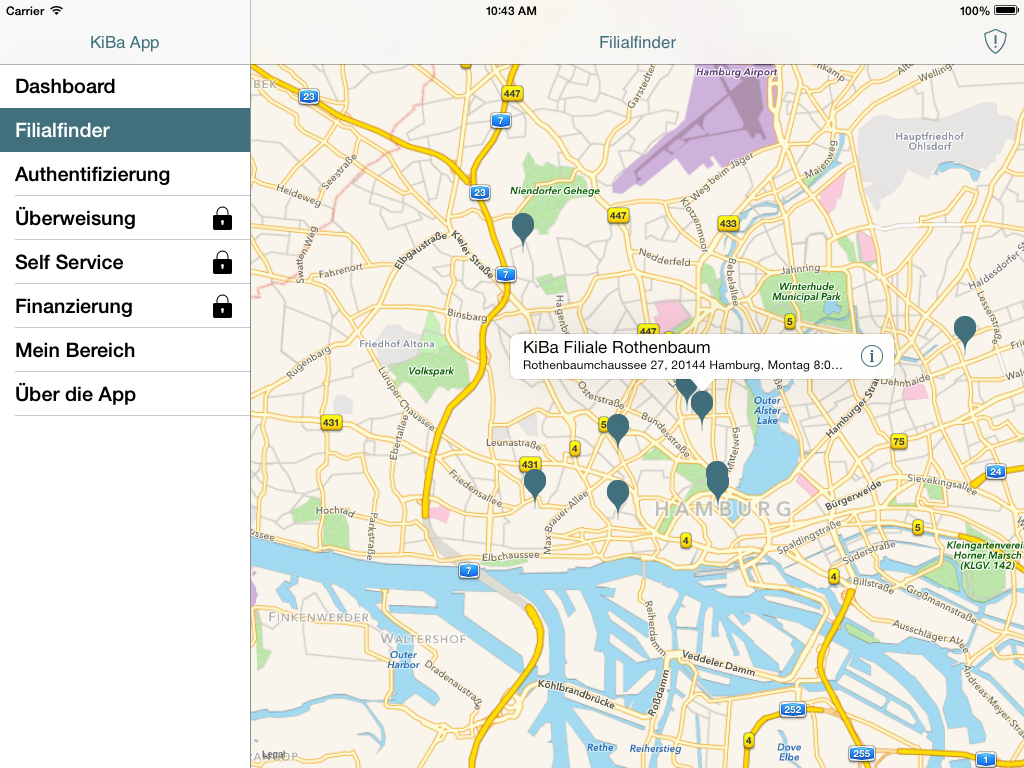
\includegraphics[height=0.25\textheight]{Pictures/filialfinder}
	\vspace{-12pt}	
	\caption{Screenshot des Filialfinders}
	\label{fig2}
\end{figure}
	Beim Filialfinder ~\ref{fig2} findet man eine Karte von Apple Maps mit Markierungen, welche die Standorte der einzelnen Filialen markieren. Mit einem Klick auf das Infosymbol gelangt man zu einer Filialseite, auf der man die Öffnungszeiten nachschauen, sowie eine Terminanfrage oder Sortenanfrage stellen kann.

\subsubsection{Sortenanfrage}
\begin{figure}[h!]
	\centering
	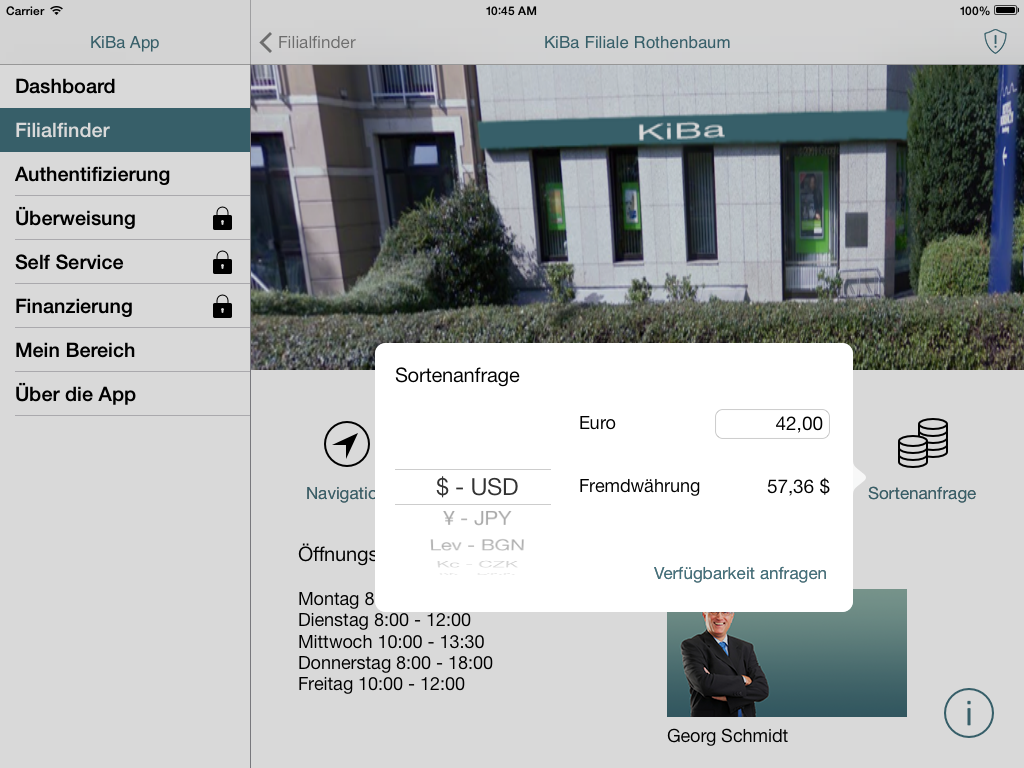
\includegraphics[height=0.25\textheight]{Pictures/Sortenanfrage}
	\vspace{-12pt}
	\caption{Screenshot der Filialseite mit Sortenanfrage Pop-Over}
	\label{fig3}
\end{figure}
	Mit einem Klick auf Sortenanfrage bekommt der Nutzer ein Pop-Over zu sehen ~\ref{fig3}, in welchem er seine Wunschwährung auswählen kann. Die entsprechenden Umrechnungskurse werden intern direkt von der Europäischen Zentralbank bezogen. Hat man die Summe, welche umgetauscht werden soll eingegeben, so kann man die Anfrage stellen und bekommt eine Nachricht, ob die gewünschte Währung in der entsprechenden Höhe bei der Filiale verfügbar ist.

\subsubsection{Authentifizierung}
\begin{figure}[h!]
    \centering
	\begin{tabular}{@{}cc@{}}
        	
\includegraphics[width=1.5cm]{Pictures/notauth} &
    		
\includegraphics[width=1.5cm]{Pictures/authed}
    \end{tabular}
	\caption{Die Authentifizierungsstati\label{fig4}}
\end{figure}
\noindent	Im oberen rechten Rand der Applikation ist ein kleines Symbol in Form eines Schildes zu sehen; dieses gibt den Authentifizierungsstatus zurück ~\ref{fig4}. Ein Schild mit einem Ausrufezeichen symbolisiert eine fehlende Authentifizierung. Ein Haken signalisiert eine gültige Authentifizierung.

	Solange das Gerät nicht authentifiziert ist, kann man einige Funktionen nicht benutzen, diese sind durch das Symbol eines ungeöffneten Schlosses gekennzeichnet.

	Unter dem Menüpunkt Authentifizierung findet man ein kleines Comic vor. Dieses erläutert, wie der Nutzer sein Gerät bei seiner Filiale authentifizieren kann. Außerdem wird der Nutzer auf seine Vorteile aufmerksam gemacht.

\subsubsection{Überweisung}
	Unter dem Menüpunkt Überweisung findet man ein Überweisungsformular in digitaler Form vor. Nachdem das Formular ausgefüllt ist, muss die Überweisung abschließend mit einer TAN bestätigt werden. Kontonummer und Bankleitzahl werden im Zuge dessen auf Korrektheit ihres Formats geprüft.

\subsubsection{Self-Service-Station}
\begin{figure}[h]
	\centering
  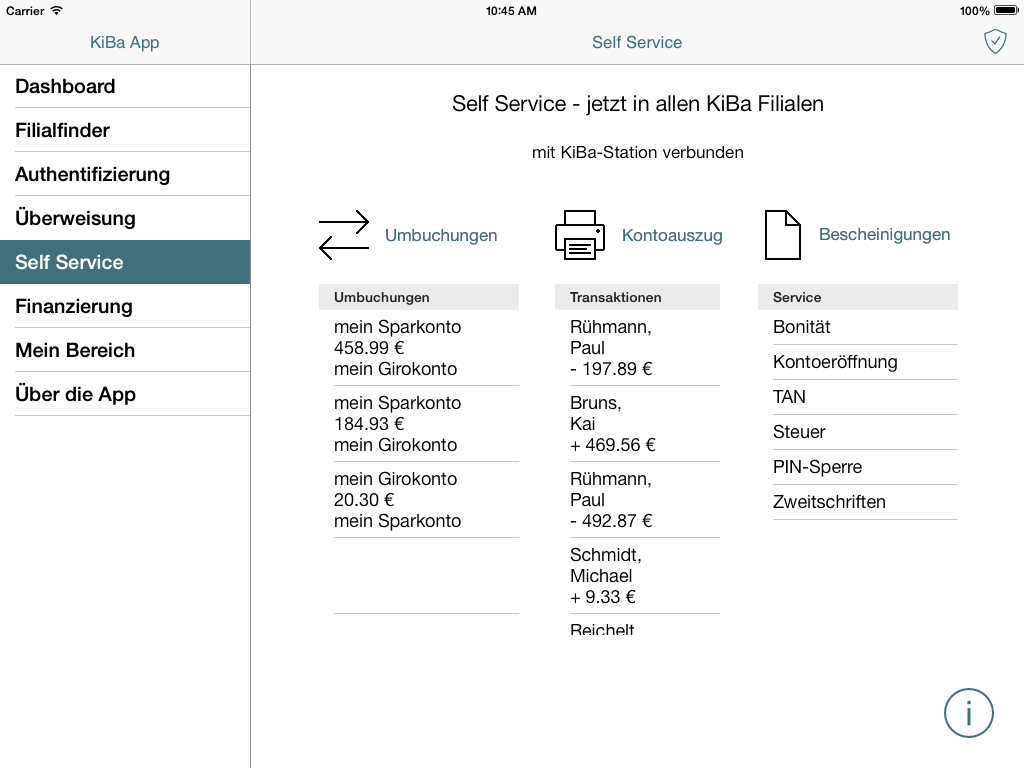
\includegraphics[width=0.5\textwidth]{Pictures/SSverbunden}
	\caption{Self-Service Startseite. Die App ist verbunden.}
	\label{fig5}
\end{figure}

\noindent	Bei der Self-Service-Station ~\ref{fig5} haben wir die Möglichkeit, sofern wir mit dem Stationsgerät verbunden sind, drei verschiedene Aktionen eigenständig durchzuführen. Eine Umbuchung, Kontoauszüge anschauen und drucken, sowie Bescheinigungen ansehen, ausfüllen und ausdrucken, gegebenenfalls direkt abschicken.

	Jede Auswahlmöglichkeit hat eine Tabelle mit Inhalten, die den User erwarten, wenn er auf den entsprechenden Button drückt.

\subsubsection{Bescheinigungen}
\begin{figure}[h!]
	\centering
  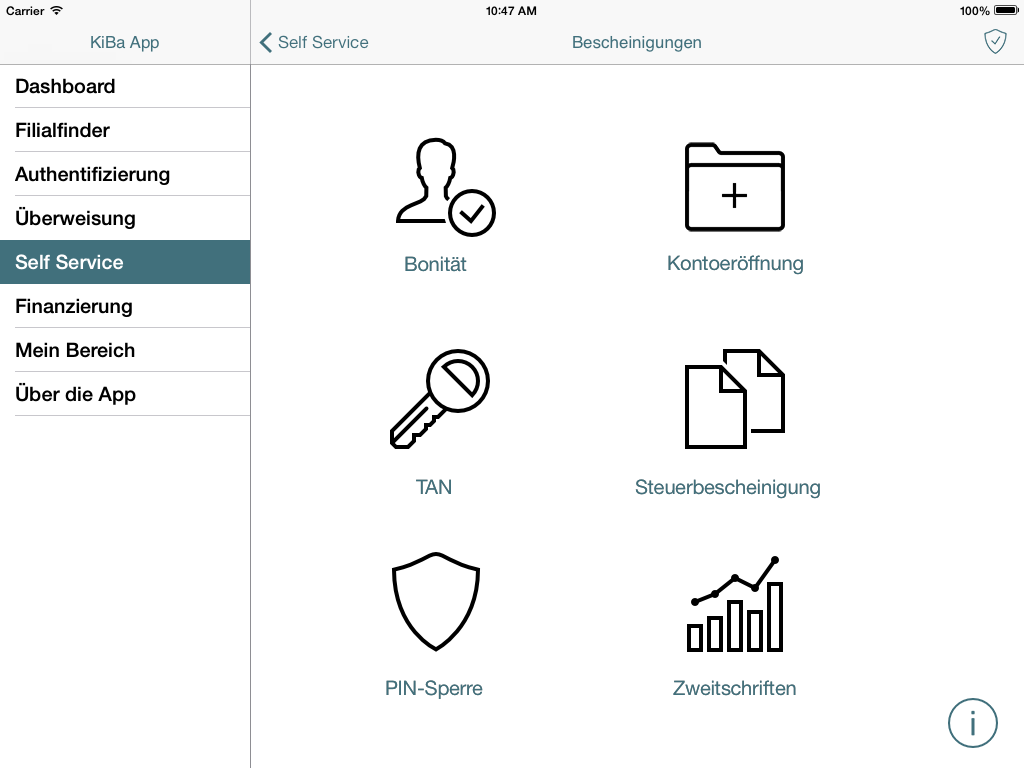
\includegraphics[width=0.5\textwidth]{Pictures/Bescheinigungen}
	\caption{Die verschiedenen Dokumenttypen}
	\label{fig6}
\end{figure}

	Bei den Bescheinigungen ~\ref{fig6} sehen wir verschiedene von der Bank zur Verfügung gestellte Dokumente, die der Nutzer auswählen kann. Insbesondere sind Aktionen wie eine Kontoeröffnung möglich, für die man normalerweise am Schalter anstehen müsste. Diese Funktionalität wurde nicht komplett implementiert, so aber die Idee andeuten die dahinter steht. Es wird beim Drücken von den Buttons nichts passieren.

\pagebreak
\subsubsection{Kontoauszüge}
\begin{figure}[h!]
	\centering
  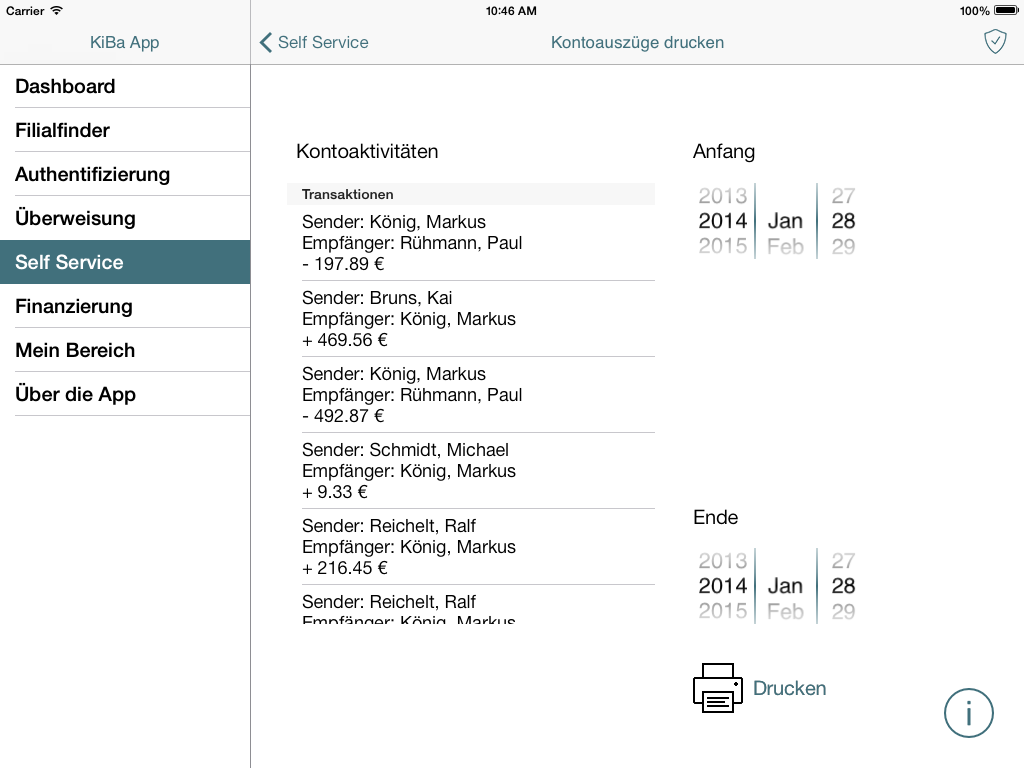
\includegraphics[width=0.5\textwidth]{Pictures/kontoauszuege}
	\caption{Übersicht der Kontoauszüge}
	\label{fig7}
\end{figure}

	Im Kontoauszugsbildschirm ~\ref{fig7} kann man Kontoaktivitäten für einen bestimmten Zeitraum drucken lassen. Somit integriert die Station den althergebrachten Kontoauszugsdrucker und gibt ihm eine zeitgemäßere Oberfläche. Die Druckfunktion ist hier auch nur angedeutet.


\subsubsection{Umbuchungen}
\begin{figure}[h!]
	\centering
  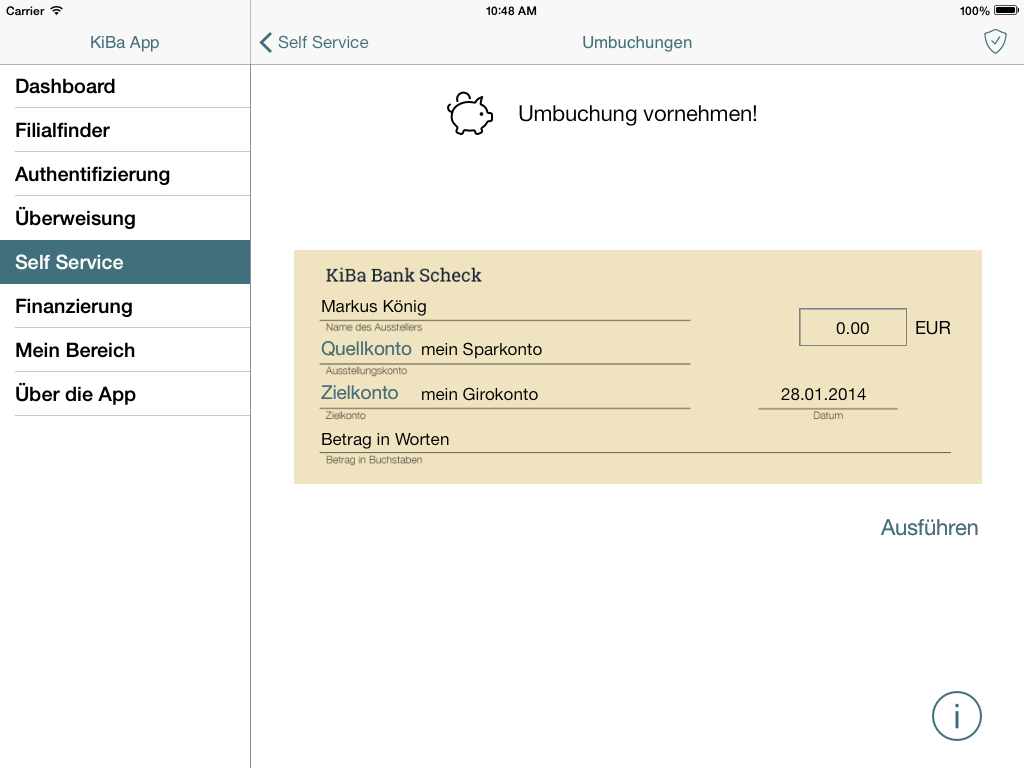
\includegraphics[width=0.5\textwidth]{Pictures/umbuchung}
	\caption{Eine Scheckgrafik als Formular für die Umbuchung}
	\label{fig8}
\end{figure}

	Im Umbuchungsbildschirm ~\ref{fig8} kann der Nutzer sowohl Ziel- als auch Quellkonto auswählen, zwischen denen der angegebene Betrag transferiert werden soll. Das Ganze wird mit einem Button bestätigt. Insbesondere wird hier das klassische Sparbuch um eine komfortable Umbuchungsfunktionalität erweitert. Umbuchungen werden weiterhin in den Räumlichkeiten der Bank vorgenommen, weshalb der filialgebundene Charakter erhalten bleibt.
\subsubsection{Finanzierungsrechner}
\begin{figure}[h!]
	\centering
  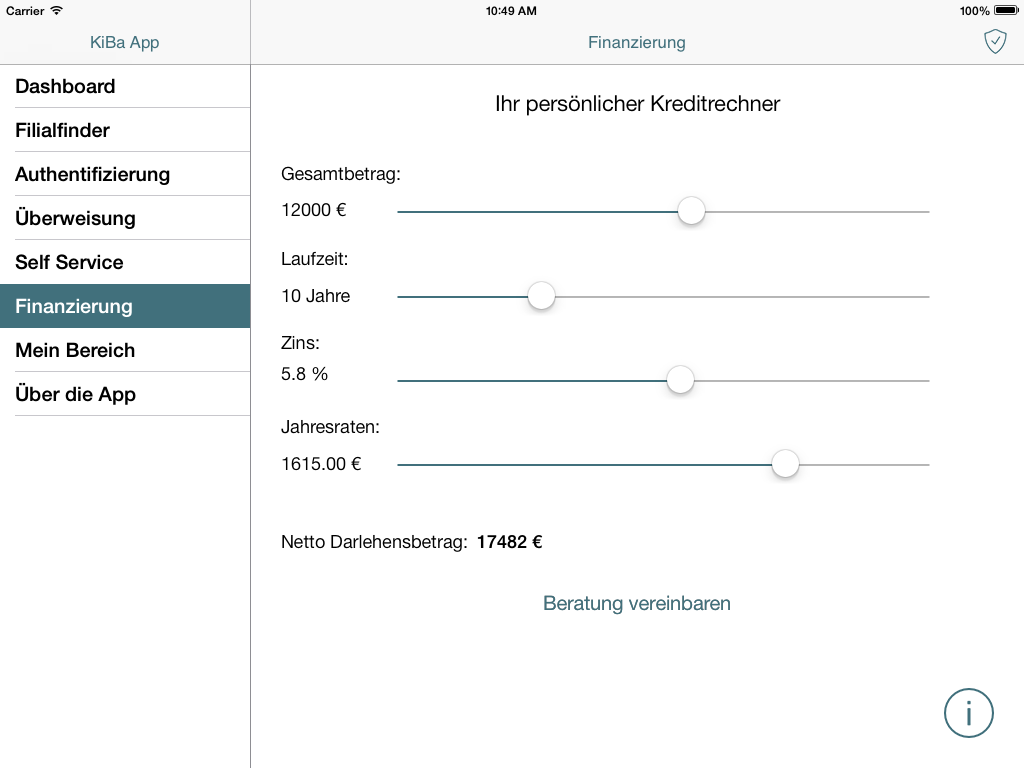
\includegraphics[width=0.5\textwidth]{Pictures/finanzierung}
	\caption{Finanzierungsrechner mit individuellen Konditionen}
	\label{fig9}
\end{figure}

	Mit dem Finanzierungsrechner ~\ref{fig9} kann man sich Kreditkonditionen zusammenstellen. Die Werte der einzelnen Schieberegler werden aus dem Profil des Kundens von der Bank vorgegeben.

	Anschließend kann man einen Beratungstermin vereinbaren, um die Konditionen mit seinem Berater im Detail durchsprechen zu können. Im Rahmen des Gesprächs bietet sich die Möglichkeit zu prüfen, inwiefern die ausgewählten Konditionen empfehlenswert für den Kunden sind oder ob die Bank vielleicht noch bessere Konditionen anbieten kann.
\pagebreak
\subsubsection{Mein Bereich}
%Nachrichtensystem
%mbereichneu.png

\begin{figure}[h!]
	\centering
  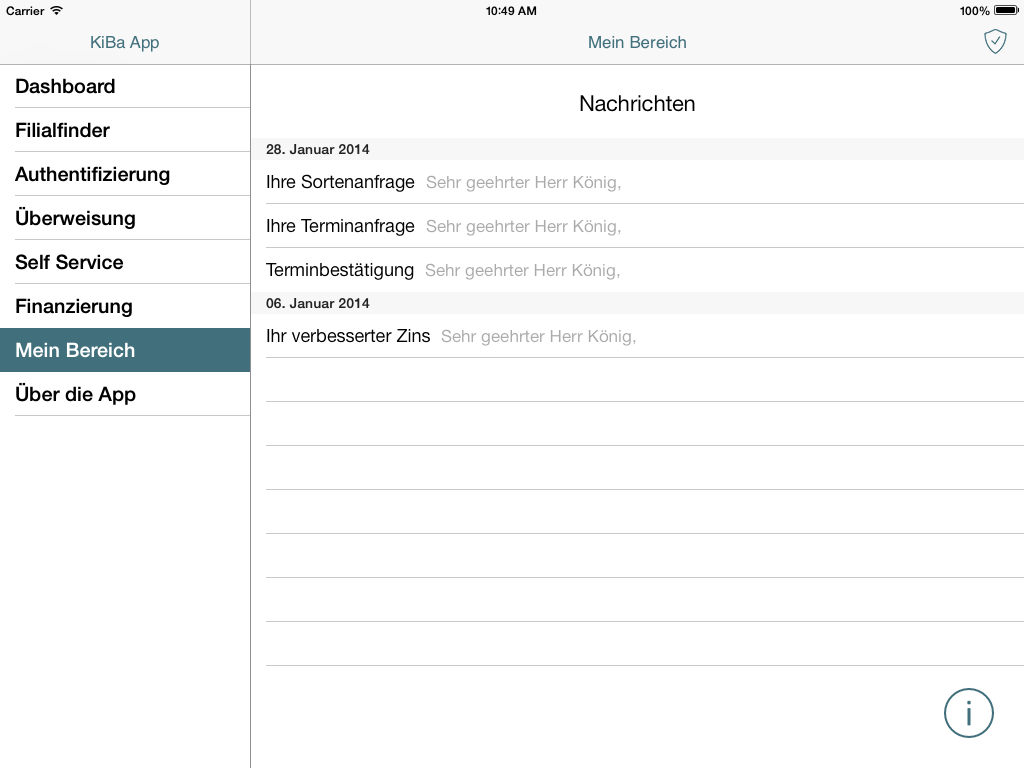
\includegraphics[width=0.5\textwidth]{Pictures/mbereichneu}
	\caption{Ein minimalistischer Posteingang des Nutzers\label{fig10}}
\end{figure}

	Der Nutzer kann in seinem persönlichen Bereich ~\ref{fig10} Nachrichten der Bank empfangen und somit beispielsweise eine Bestätigung für seine Terminanfrage erhalten. Mit einem Klick auf die Zelle einer Nachricht bekommt man die entsprechende Nachricht in einer neuen Ansicht mit dem kompletten Nachrichtentext.
\subsection{Die Design-Highlights}
\begin{figure}[h!]
	\centering
    \begin{tabular}{@{}ccc@{}}
    		\framebox{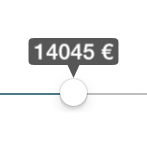
\includegraphics[width=2.5cm]{Pictures/DesignA}} &
    		\framebox{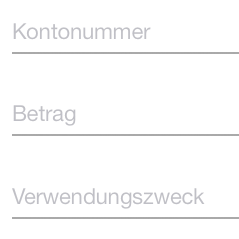
\includegraphics[width=2.5cm]{Pictures/DesignC}} &
    		\framebox{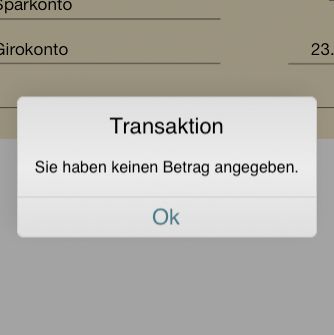
\includegraphics[width=2.5cm]{Pictures/DesignB}} \\
    		A & B & C
    \end{tabular}
	\caption{Eigenkreationen für das Design\label{fig11}}
\end{figure}

Um unsere Applikation in mancher Hinsicht besser auf unsere Bedürfnisse anzupassen, haben wir bei einigen Designelementen die Standardimplementierungen von Apple ergänzt. Dennoch blieben die iOS 7 Richtlinien ein Qualitätsmaßstab für uns.

Wie in ~\ref{fig11} zu sehen ist, bekam unser Schieberegler als kleine Erweiterung eine schwarze Sprechblase, welche den aktuellen Wert anzeigt. Dies ist im Speziellen unter dem Gesichtspunkt der Bedienbarkeit implementiert worden, damit man beim Verschieben des Reglers nicht immer auf die linke Seite schauen muss, um den aktuellen Wert abzulesen.

Die mitgegebenen Textfelder von Apple haben in der Regel immer einen Text, welcher dem Nutzer einen Hinweis gibt, was für ein Inhalt erwartet wird. Diese Umsetzung sieht oftmals unschön aus und nimmt viel Platz ein. Mit unserer Implementierung ~\ref{fig11} verliert das Textfeld keine Funktionalität, ist aber schlanker.

Die Standard Pop-Over lassen sich nur bedingt anpassen. So konnten wir die Farbe des Buttons nicht in unserem Farbton einfärben. Daher mussten wir auf eine Eigenimplementation ~\ref{fig11} zurückgreifen um die Konsistenz zu wahren.


\subsection{Herausforderungen}
	Mit zu den größten Herausforderungen war das Design der einzelnen Bildschirme. Das „Flat“-Design braucht ein gutes Händchen und kleine Details können schon zu Unstimmigkeiten führen. Gleichzeitig war uns bewusst, dass wir eine Bank repräsentieren und somit ein gewisses Maß an Seriosität erforderlich war. Gleichzeitig mussten wir die Usability für den Endnutzer gewährleisten. Wir mussten ein App-Design erschaffen, welches drei Stakeholder gleichzeitig zufriedenstellt.

	Mit einer neu zu erlernenden Programmiersprache und deren Entwicklungsumgebung geht auch immer eine Herausforderung einher. Die ersten Wochen hatten wir somit erwartungsgemäß etwas geringere Produktivität, weil wir uns auf diese Gegebenheiten erst einstellen mussten. Je weiter jedoch das Projekt voranschritt, desto sicherer fühlten wir uns in Objective-C und im Umgang mit Xcode.

	Während der Entwicklung stießen wir immer wieder auf Einschränkungen seitens Apple bezüglich der Standard GUI-Elemente. So konnten wir beispielsweise die Tint-Color eines Buttons im Pop-Over nicht ändern. Wie erwähnt griffen wir, falls nötig, in diesen Fällen auf Eigenimplementationen zurück.
	
	Darüber hinaus wollten wir gewährleisten, dass die GUI-Elemente unserer Applikation, sowohl in der Potrait-Ansicht, als auch in der Landscape-Ansicht gut gesetzt sind. Dafür haben wir in den meisten Fällen die Auto-Layout-Technik verwendet. Die Verhältnisse und Größen der Elemente werden dabei mit Hilfe von Constraints beschrieben. Ändert sich das Ansichtsformat, passen sich diese dynamisch an die neuen Gegebenheiten an.
	
	Bei einigen Features überdeckte die hereinfahrende Tastatur das vom Nutzer ausgewählte Eingabefeld. Anstatt die Anordnung der Elemente der einzelnen Bildschirme zu verändern, haben wir dynamische Scrollviews in das Projekt integriert. Diese reagieren stets so, dass sich das vom Nutzer fokussierte Element möglichst zentral im freien Sichtbereich befindet.

	Zusammenfassend betrachtet konnten wir mit Unterstützung der Betreuer, alle größeren und kleineren Herausforderungen bewältigen und hatten nie das Gefühl, vor einem unüberwindbaren Problem zu stehen.
	
	
\authoredSection{markus}{Architektur}
	Nachdem zunächst in diesem Bericht bereits Konzepte und Ergebnisse erläutert wurden gehen wir an dieser Stelle nun auf die Implementierung und technische Umsetzung der App ein. Im Fokus dabei steht die Architektur, die maßgeblich zum Ablauf der Entwicklung und zur Organisation der Kernkomponenten beiträgt.
	
	Unsere App soll den Kontakt zwischen einer Filialbank und seinen Kunden stärken. Da es sich bei KiBa lediglich um eine fiktive Bank handelt und die App auch anderen interessierten Banken vorgestellt werden soll, bietet es sich an, einen "Click-Dummy" zu entwickeln. Dieser soll sich bereits wie eine vollwertige Banking-App bedienen lassen, die jedoch an keine reale Bank, respektive deren Datenbank, angeschlossen ist. Aufgrund dieser Rahmenbedingungen, haben wir uns für die Architektur entschieden, die im Folgenden vorgestellt wird.

\subsection{Umsetzung des MVC-Ansatzes}
	Die Architektur muss uns dabei auf die Entwicklung der Kernfeatures fokussieren. Wenn nicht klar ist, welche Teile der Logik, der GUI oder anderer 

\subsection{Datenmodell}
	

\subsection{Datenübertragung}
\begin{itemize}
	\item keine Speicherung auf dem Gerät (Sicherheit)
	\item alle Daten werden direkt übertragen
	\item die Datenquelle soll leicht angepasst werden können über Dependency Injection
\end{itemize}

\subsection{Dependency Injection}
	Eine zentrale Anforderung der App-Architektur für uns ist außerdem das Austauschen von einzelnen Kernkomponenten, wie etwa die Datenschicht. Denn hierdurch kann aus dem Click-Dummy eine vollwertige Banking-App erschaffen werden können, ohne große Änderungen am Code vornehmen zu müssen.  Sie muss uns den Eindruck nehmen können, an eine echte Bank gebunden zu sein.
	
	Die Abstraktion der Datenschicht sollte das Testen der App auch erleichtern. Dadurch, dass in dem Click-Dummy feste Daten hinterlegt sind, kann man sich zum Testen der App eine Authentifizierung gegenüber der Bank und das Warten auf die Datenübertragung sparen. Alle 
	
\begin{itemize}
	\item um einzelne Komponenten leicht austauschen zu können (hauptsächlich die Datenschicht)
	\item Abhängigkeiten sind an einem zentralen Ort geregelt (Bootstrap)
	\item ist nur eine Art Dependency Injection, weil unsere Klassen die Instanzen selber holen, der Dependency Manager gibt nur die richtige Instanz zurück
\end{itemize}
\authoredSection{corny}{Toolchain}
Im Rahmen unseres Projekts wurde uns schnell klar, dass wir auf viele Tools angewiesen sein würden. So musste unser Quelltext versioniert, die grobe Struktur und Views festgehalten und Aufgabenpakete erstellt und koordiniert werden. Darüber hinaus waren uns auch Design und Qualität wichtig. Auf unsere Erfahrungen in diesem Zusammenhang gehen wir im folgenden Abschnitt ein.

\subsection{Agiles Vorgehen im Projekt}
	Da uns freundlicherweise von der C1 WPS GmbH die Möglichkeit gegeben wurde, eine Scrum-Zer\-ti\-fi\-zie\-rung zu erhalten, lag uns viel daran, den Scrum-Ansatz so gut es ging in unseren Projekt-Ablauf zu integrieren. Zudem war es im Rahmen der wöchentlichen Projektdiskussion Vorgabe, den Fortschritt anhand eines Scrum-Tools dokumentiren zu können.
	
	Dazu verwendeten wir – nach ersten Versuchen mit GitHub-Issues – die Software PivotalTracker. Während GitHub zwar eine für andere Zwecke ausreichende Möglichkeit bietet, sogenannte Issues anzulegen und abzuarbeiten, kann PivotalTracker den gesamten Scrum-Ablauf abbulden.
	Beispielsweise können wir, wie in Abbildung \ref{fig:TrackerStories} dargestellt, einzelne Stories erstellen und überwachen. Ein großer Vorteil dabei war, dass Scrum-Iterationen automatisch von der Software generiert werden, berechnet durch unsere durchschnittliche Arbeitskraft (genannt „Velocity“)\footnote{\url{http://www.pivotaltracker.com/community/tracker-blog/velocity-matters}} und unseren Vorhersagen für den Aufwand einer Story angegeben durch Punkte.
	
\begin{figure}[h!]
	\centering
	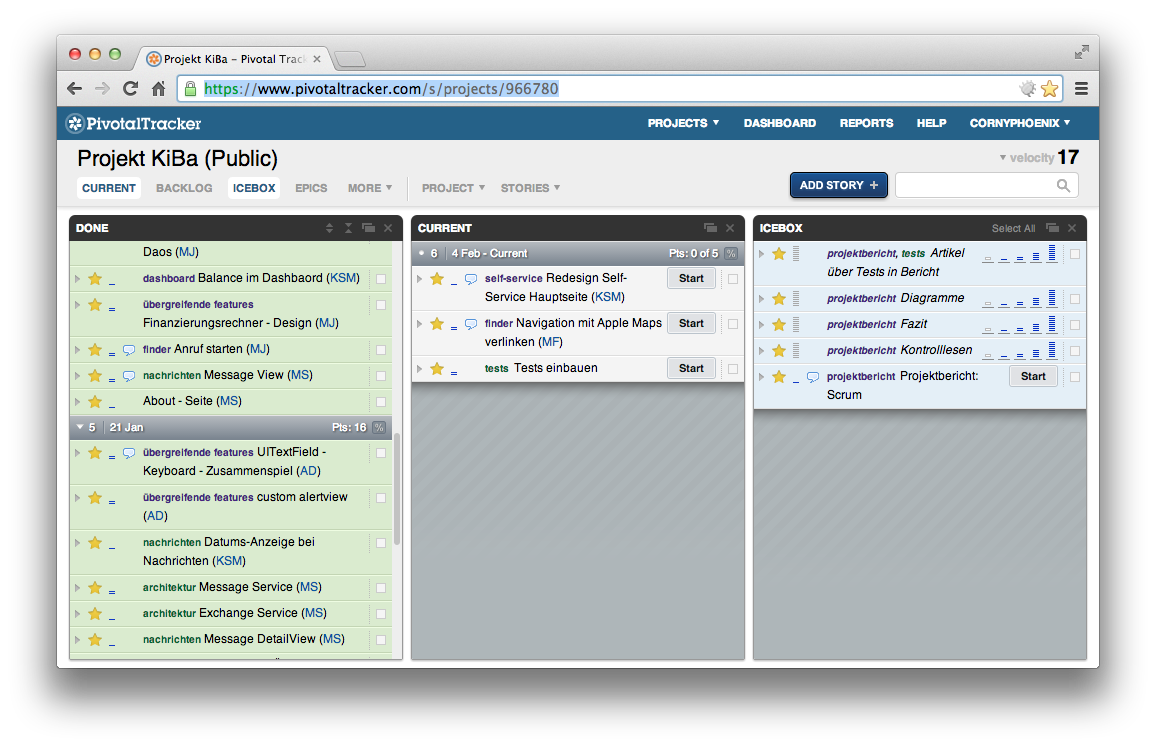
\includegraphics[scale=.25]{Pictures/TrackerStories}
	\vspace{-.8cm}
	\caption{Stories in PivotalTracker\label{fig:TrackerStories}}
\end{figure}

\noindent	Zum anderen generiert PivotalTracker auch Burndown-Charts, welche für das Vorgehen während der Scrum-Iterationen unabdinglich sind. Denn so können wir am besten den Fortschritt unserer App messen und haben ein Monitoring für das Fortschreiten der Entwicklung unserer Features, wie in Abbildung \ref{fig:TrackerBurndown} zu sehen ist.

\begin{figure}[h]
	\centering
	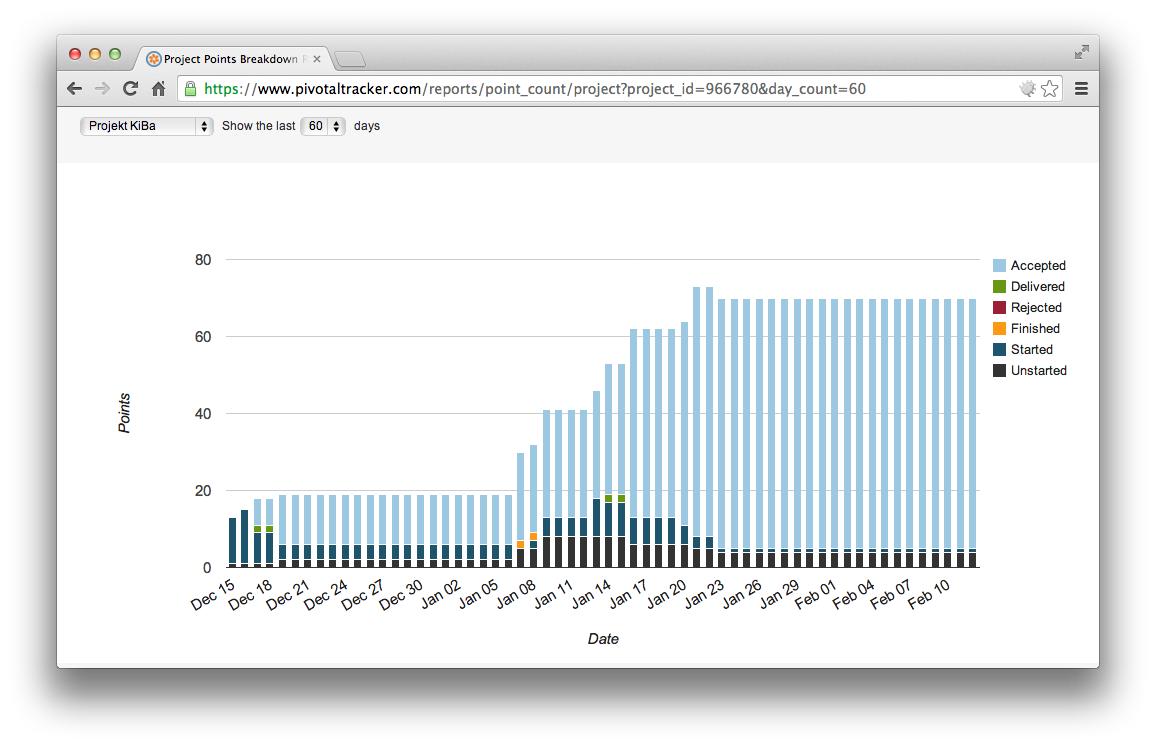
\includegraphics[scale=.25]{Pictures/TrackerBurndown}
	\vspace{-.8cm}
	\caption{Burndown-Chart in PivotalTracker\label{fig:TrackerBurndown}}
\end{figure}

\subsection{Versionsverwaltung und Informationsaustausch}
	Um kollaborativ an einer Software zu arbeiten, ist es selbstverständlich erforderlich, mit Quelltextversionierung zu arbeiten. Da bei uns Team-Mitgliedern die Erfahrung mit Git\footnote{\url{http://git-scm.com/}} aus dem Universitäts- und Arbeitsumfeld am größten war, fiel unsere Wahl für ein \acs{VCS} darauf. Entscheidend dabei war auch der größere Komfort gegenüber Subversion und die Möglichkeit, die Plattform GitHub\footnote{\url{https://github.com/}} als Repository-Hoster und anfangs auch als Issue-Tracker zu verwenden. Wie unser Repository bei GitHub aussieht, ist in Abbildung \ref{fig:GitHubOverview} zu sehen.
	
	Ein weiteres nützliches Feature von GitHub für uns war außerdem ein Wiki, dargestellt in Abbildung \ref{fig:GitHubWiki}. In ihm tauschen wir Informationen aus, wie beispielsweise erste Feature-Ideen oder Kontaktdaten aller Mitglieder. Allerdings nutzten wir es darüber hinaus auch für das Festlegen eines Arbeitsablaufs mit Xcode.
	
\begin{figure}
	\centering
	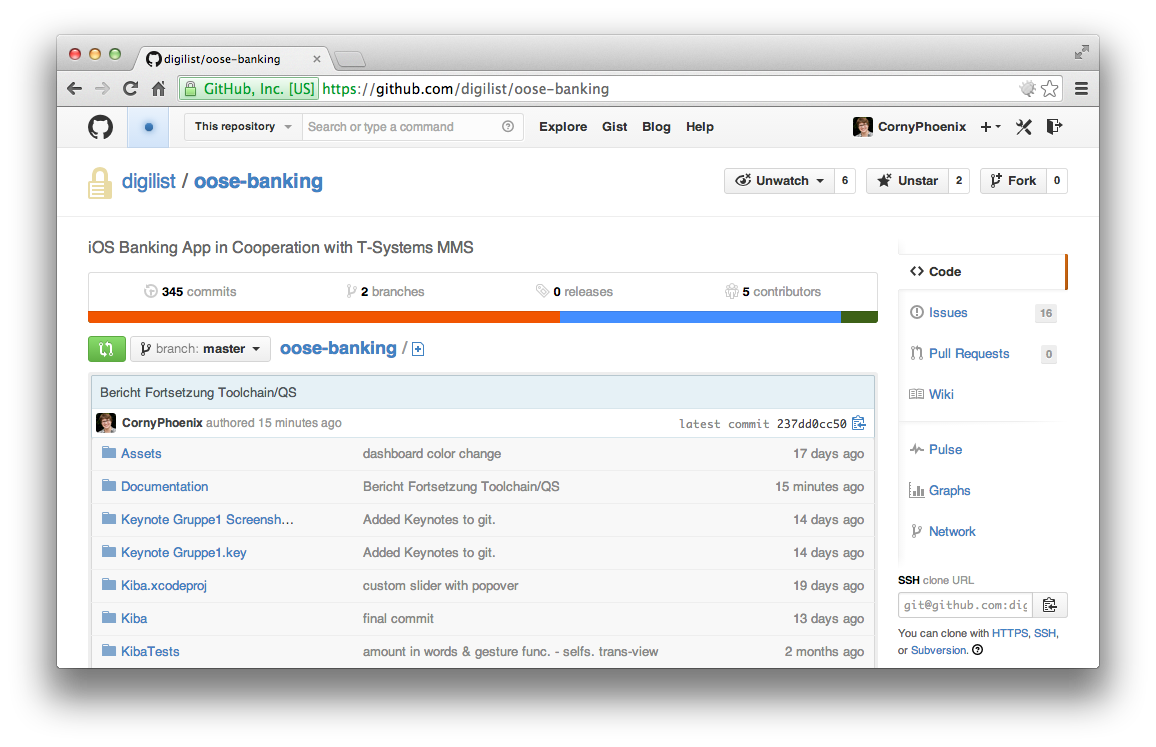
\includegraphics[scale=.25]{Pictures/GitHubOverview}
	\caption{Quelltext-Hosting bei GitHub \label{fig:GitHubOverview}}
\end{figure}

\begin{figure}
	\centering
	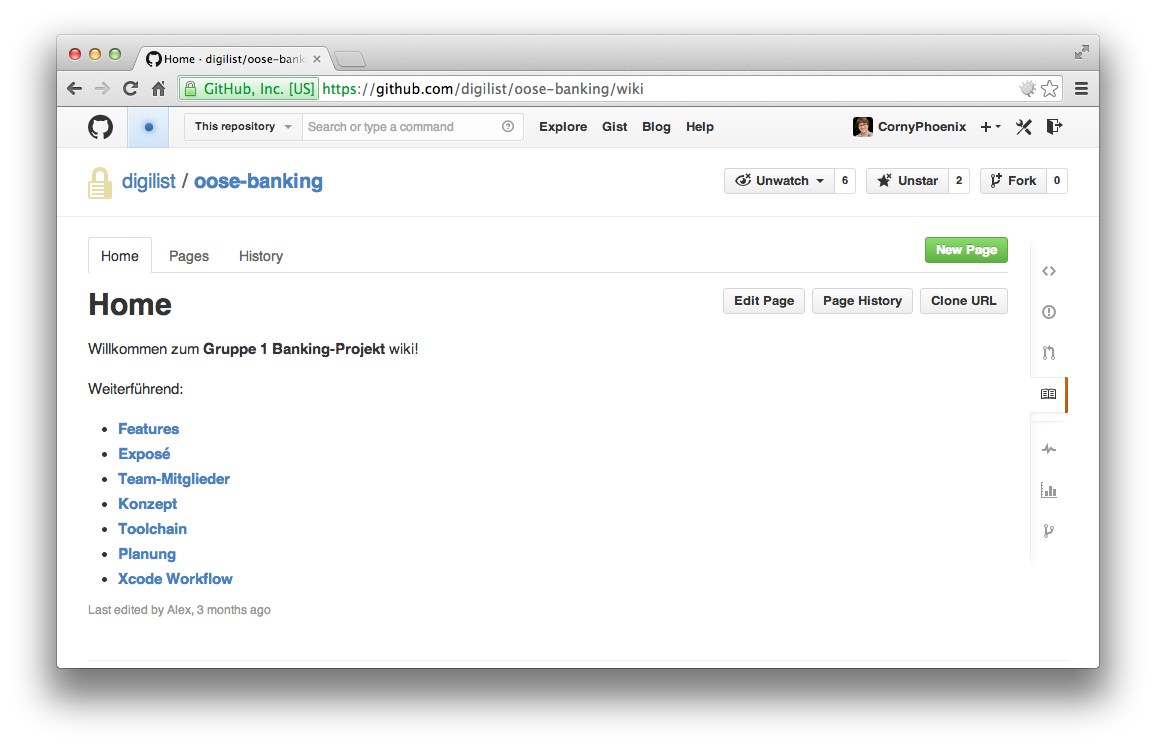
\includegraphics[scale=.25]{Pictures/GitHubWiki}
	\caption{GitHub-Wiki für den Wissensaustausch \label{fig:GitHubWiki}}
\end{figure}

\subsection{Konzept und erster Entwurf}
Balsamiq
\begin{figure}
	\centering
	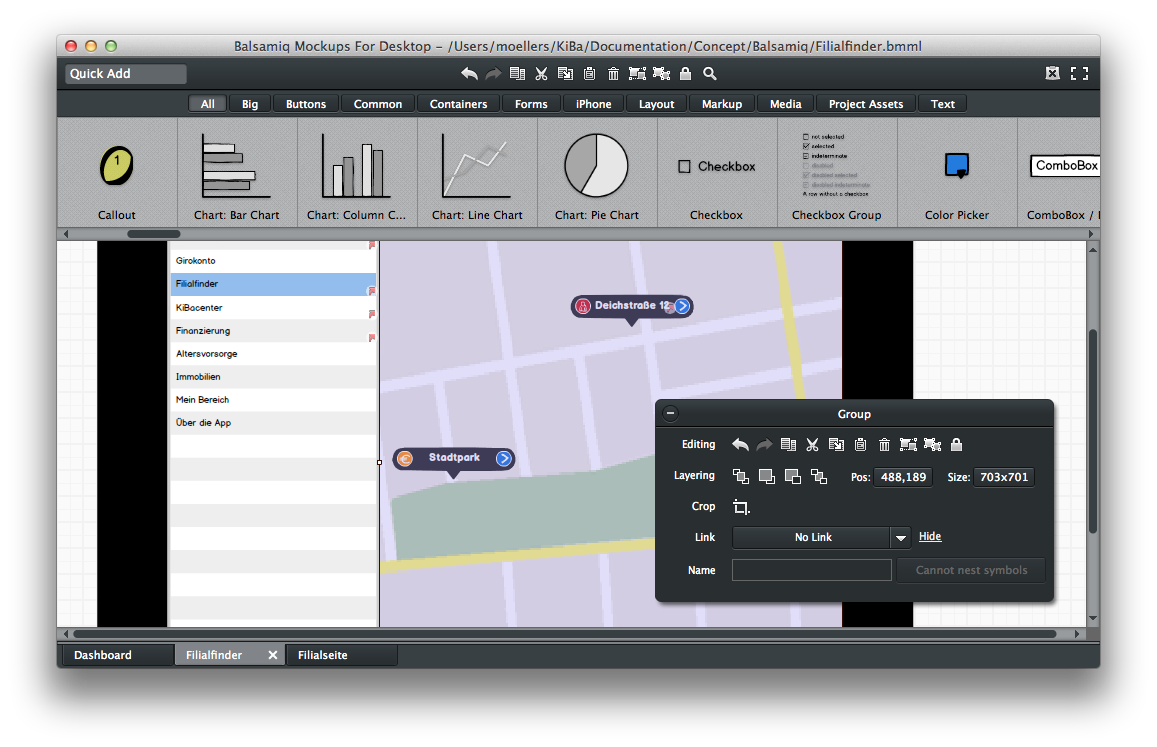
\includegraphics[scale=.3]{Pictures/BalsamiqEntwurf}
	\label{fig:BalsamiqEntwurf}
	\caption{Entwerfen mit Balsamiq}
\end{figure}

\subsection{Designtools}
Adobe Illustrator/Photoshop
\begin{figure}
	\centering
	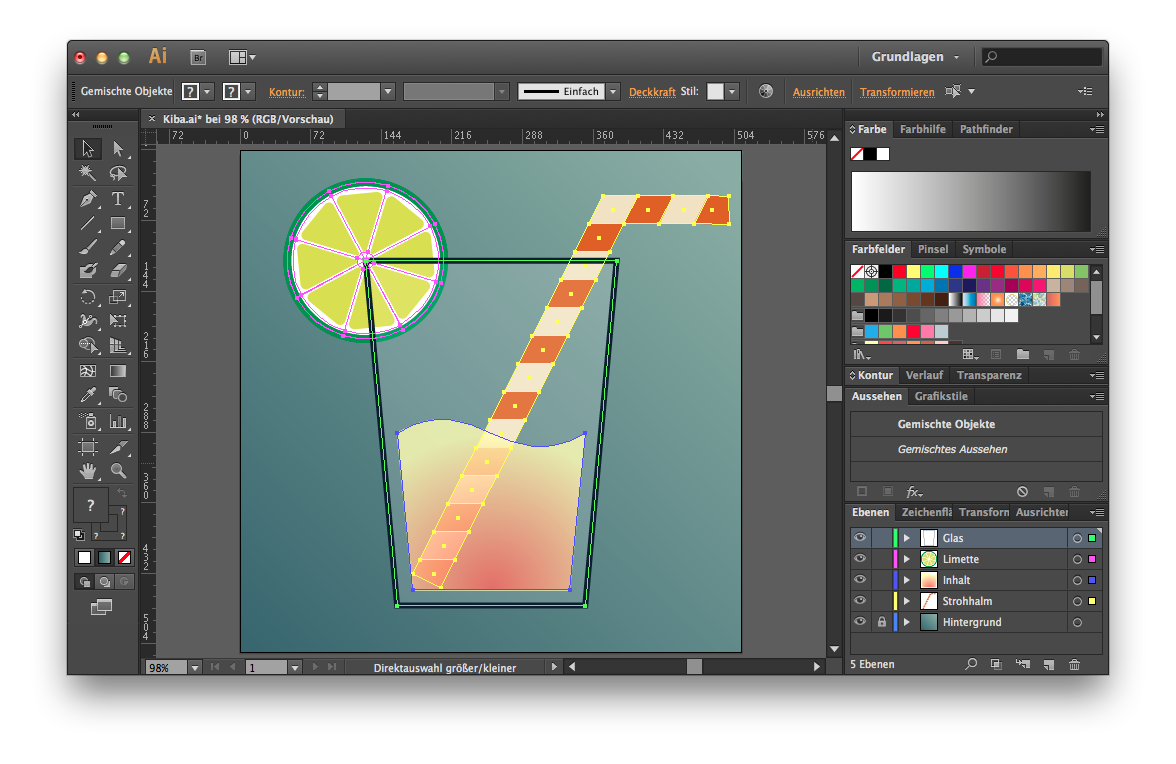
\includegraphics[scale=.3]{Pictures/IllustratorIcon}
	\label{fig:IllustratorIcon}
	\caption{Designen des KiBa-Icons mit Adobe Illustrator}
\end{figure}
\authoredSection{corny}{Qualitätssicherung}
	Für große Projekte wird es zunehmend unabdinglich, über Planung und Ausführung hinaus auch ein Monitoring und Controlling zu besitzen, auf welche ich in Form der Qualitätssicherung in diesem Abschnitt eingehen werde.\footnote{\textsc{Projekt Management Institute}: \textit{A Guide to the Project Management Body of Knowledge}. Fifth Edition. Newton Square, 2008. 589 Seiten.}

\subsection{Entwicklungsprozess}
	Um Planungssicherheit zu haben benötigt man einen kontinuierlichen Prozess, damit man weiß, an wen welche Aufgaben zu verteilen sind und jeder Projektteilnehmer den Vorgangsablauf kennt. In unserem Fall war die Aufgabenverteilung bereits durch Telekom anhand der Rollen Projektmanager, Konzepter, Berater und Entwickler vorgegeben, sodass wir uns auch versuchten daran zu orientieren. 
	
	Unsere Arbeitsprozesse waren wichtig für die Qualität der Entwicklung. Die effektive Arbeitsteilung half uns, sich auf seinen Bereich fokussieren zu können und mit entsprechender Kenntnis voranschreiten zu können. Auch wenn die Umsetzung der Prozesse nicht immer absolut problemfrei ablief, so haben wir es doch geschafft, unsere beiden Hauptfeatures Finder und Self-Service gut umsetzen zu können.

\subsection{Qualität des Designs}
	Damit sichergestellt ist, dass wir ein konsistentes, qualitatives Design haben, versuchten wir uns grundlegend an den iOS7-Design-Richtlinien zu orientieren.\footnote{\url{https://developer.apple.com/library/ios/documentation/userexperience/conceptual/mobilehig/}} Da leider kein Mitglied von uns weitreichende Erfahrungen mit Design-Werkzeugen hatte, war die Umsetzung deren für uns von größerem Problem.

\subsection{Umgang mit Feedback}
	Ein effektives Instrument zur Qualitätssicherung, dass uns durch die Veranstalter zur Verfügung gestellt wurde, ist das Feedback von potentiellen Kunden. Umso mehr ist es für uns daher eine große Hilfe gewesen, dass auf Probleme und Wünsche bei der App in wöchentlichen Plenarveranstaltungen eingegangen wurde. Wir haben jedes Feedback umgehend in unserer Facebook-Gruppe dokumentiert und Lösungen ausdiskutiert.
	
	Dieser Vorgang hat uns sehr in der Einhaltung der oben geschilderten Prozesse geholfen. Da wir uns jeden Dienstag und Donnerstag im Mac-Arbeitsraum getroffen hatten, konnten wir erst neue Storys in PivotalTracker anhand des Feedbacks anlegen, diese dann unter uns aufteilen und bis zur nächsten Plenarveranstaltung abarbeiten. Man kann sagen, dass wir also die Plenarveranstaltung als „Motor“ für unsere Scrum-Iterationen benutzt haben.
	
	Wir entwickelten somit über die Zeit ein immer besseres Gefühl für die Umsetzung von Feedback und auch über die Möglichkeit, Scrum als Methode des agilen Projektmanagements anzuwenden.

\subsection{Ausblick}
	Über die vorangegangen Punkte hinaus haben wir uns außerdem überlegt, wie wir auch entwicklungstechnischer Sicht Qualitätssicherung umsetzen können. Unser nächster Schritt in der Entwicklung wäre daher auch das Einbinden von Unittests gewesen, um auch in Hinblick auf die oben beschriebene Architektur eine Absicherung über die Prozesse geben.
	
	Programmausdruck \ref{lst:Unittest} zeigt ein Beispiel für so einen Unittest, wie er die Arbeitsweise der Dependency Injection verifizieren kann. Er zeigt, wie beispielsweise das Einbinden der Authentifizierung getestet werden kann.
	
	\lstinputlisting[label={lst:Unittest}, caption={Beispiel für einen Unittest mit iOS}]{Listings/Unittest}
\authoredSection{michael}{Fazit}
	Das Projekt objektorientierte Softwareentwicklung hat für uns in gewisser Hinsicht eine Zäsur im Studium markiert. Bisherige Module oder Praktika legten den Fokus auf eine technisch möglichst saubere Implementierung, bei der im Zweifel das Interaktionsdesign oder der Funktionsumfang zurückgestellt wurden. Im Projekt wurde die Beherrschung objektorientierter Techniken bereits vorausgesetzt und erstmalig ein Software-Produkt entwickelt, das in seiner Gesamtheit auch industriellen Anforderungen genügen musste. 

	Mehrere Teilnehmer unserer Gruppe hatten bereits ein erstes Maß an Arbeitserfahrung vorzuweisen, etwa als Werkstudent oder selbständiger Webentwickler. Trotzdem wurde in den ersten Wochen des Projekts deutlich, dass im Bezug auf die Arbeitsorganisation als Auftragnehmer eines Produkts noch Raum für Verbesserungen war. 

	Dies galt insbesondere für den Umgang mit Designfragen und der Reihenfolge der Entwicklung. In einer Gruppe, die bis auf eine Ausnahme aus Informatikstudenten bestand, gingen wir zunächst in bekannter Manier vor. Um die Eigenheiten von iOS und Objective-C kennenzulernen, unternahmen wir erste Gehversuche in Funktionen wie einer Überweisungsansicht, die für das Endprodukt sekundär waren. Ebenso behandelten wir in den ersten Überlegungen das Design noch etwas stiefmütterlich. Eine Mentalität, der im Informatikstudium nicht selten Vorschub geleistet wird, ließe sich auf die Aussage „Erst wird programmiert, dann das Design nachgeschoben“ reduzieren. Im Plenum wurde uns aufgezeigt, dass ein solcher Ansatz nicht nur weniger effizient ist, sondern auch das eigene Produkt schlechter dastehen lässt. 

	Einerseits ist es in einem engen Zeitrahmen sinnvoller, sich voll und ganz auf die Funktionen zu konzentrieren, die Alleinstellungsmerkmale darstellen und den innovativen Kern des Konzepts bilden. Denn nur anhand dieser lässt sich ein Kunde von einem Produkt überzeugen. Zudem erfordert ein benutzerzentriertes Design, das erst nachträglich hinzugefügt wird, umständliche Änderungen an der Codebasis. Gleichzeitig können bereits wenige, minimalistische Designelemente in konsistenter Farbe und Anordnung einen enormen Unterschied in der Wahrnehmung der Produktqualität bedeuten.

	Entsprechend haben wir unsere Arbeitsweise adjustiert und ein neues Verständnis von zeitgemäßer Softwareentwicklung gewonnen. Während innovative Funktionalität von technischer Seite weiter geboten ist, hat sich der Anspruch der Benutzer an die Bedienbarkeit stark gewandelt; Apps, die dies nicht berücksichtigen, haben auf einem derart umkämpften Markt wenig Erfolgsaussicht.


\newpage

%===============================================================================
% Verzeichnisse
%===============================================================================
\renewcommand{\currentAuthor}{kiba}
\phantomsection
\addcontentsline{toc}{section}{Abbildungsverzeichnis}
\listoffigures


\end{document}